This chapter summarizes the key findings of the proposed methods for vehicle space occupancy estimation under low-light conditions. It provides a comparative evaluation of the approaches introduced, highlighting their strengths, limitations, and suitability for different scenarios.
\begin{itemize}
    \item \textbf{Method 1} relies on a homography computed from four coplanar vehicle points. While it is simple and computationally efficient, it heavily depends on strong perspective cues. When these cues are weak or absent—such as in frontal or rear views—the method often fails to recover a meaningful pose, limiting its applicability in real-world scenarios.
    \item \textbf{Method 2} builds upon geometric reasoning using vanishing points to estimate the angle between back-projected rays of the two taillights. This method demonstrates high accuracy and reliability when vanishing points can be reliably detected. It avoids strong planar assumptions and performs well under a wide range of perspectives. However, its dependence on precise line detection and vanishing point localization can become a weakness in low-resolution or cluttered images.
    \item \textbf{Method 3} introduces a more sophisticated and iterative approach, reducing the 3D-to-2D problem to a 2D-to-1D projection and refining pose estimates using known vehicle dimensions. It proves to be one of the most robust methods, especially under weak perspective conditions where other methods struggle. Its ability to recover accurate poses from minimal cues makes it highly suitable for real-world deployment. The trade-off lies in the increased computational complexity and reliance on iterative refinement.
    \item \textbf{Method 4} uses the Perspective-n-Point (PnP) framework to estimate vehicle pose from known 3D-to-2D correspondences. While it is highly flexible and accurate when accurate correspondences are available, its performance is sensitive to point detection quality and the assumption of correct vehicle geometry. Additionally, it may not perform well when all visible points lie on the same plane, causing pose ambiguity.
\end{itemize}

In summary, Methods 2 and 3 offer the best balance between accuracy and robustness. Method 2 excels when vanishing points are well-defined, while Method 3 provides resilience in more ambiguous scenes. Methods 1 and 4, although useful in specific contexts, face limitations in generalizability and reliability. Future work may explore hybrid approaches that combine vanishing point geometry with iterative refinement for even greater performance in diverse environments.

\section{Comparison of Results}
The figure \ref{fig:grid_images} shows the comparison between the implemented methods across different frames.

\begin{figure}[htbp]
    \centering
    \setlength{\tabcolsep}{5pt} % column spacing
    \renewcommand{\arraystretch}{1.1} % row height
    \begin{tabular}{c c c c c}
        & \textbf{Frame 4} & \textbf{Frame 8} & \textbf{Frame 12} & \textbf{Frame 16} \\[5pt]

        \raisebox{9\height}{\textbf{Method 1}} &
        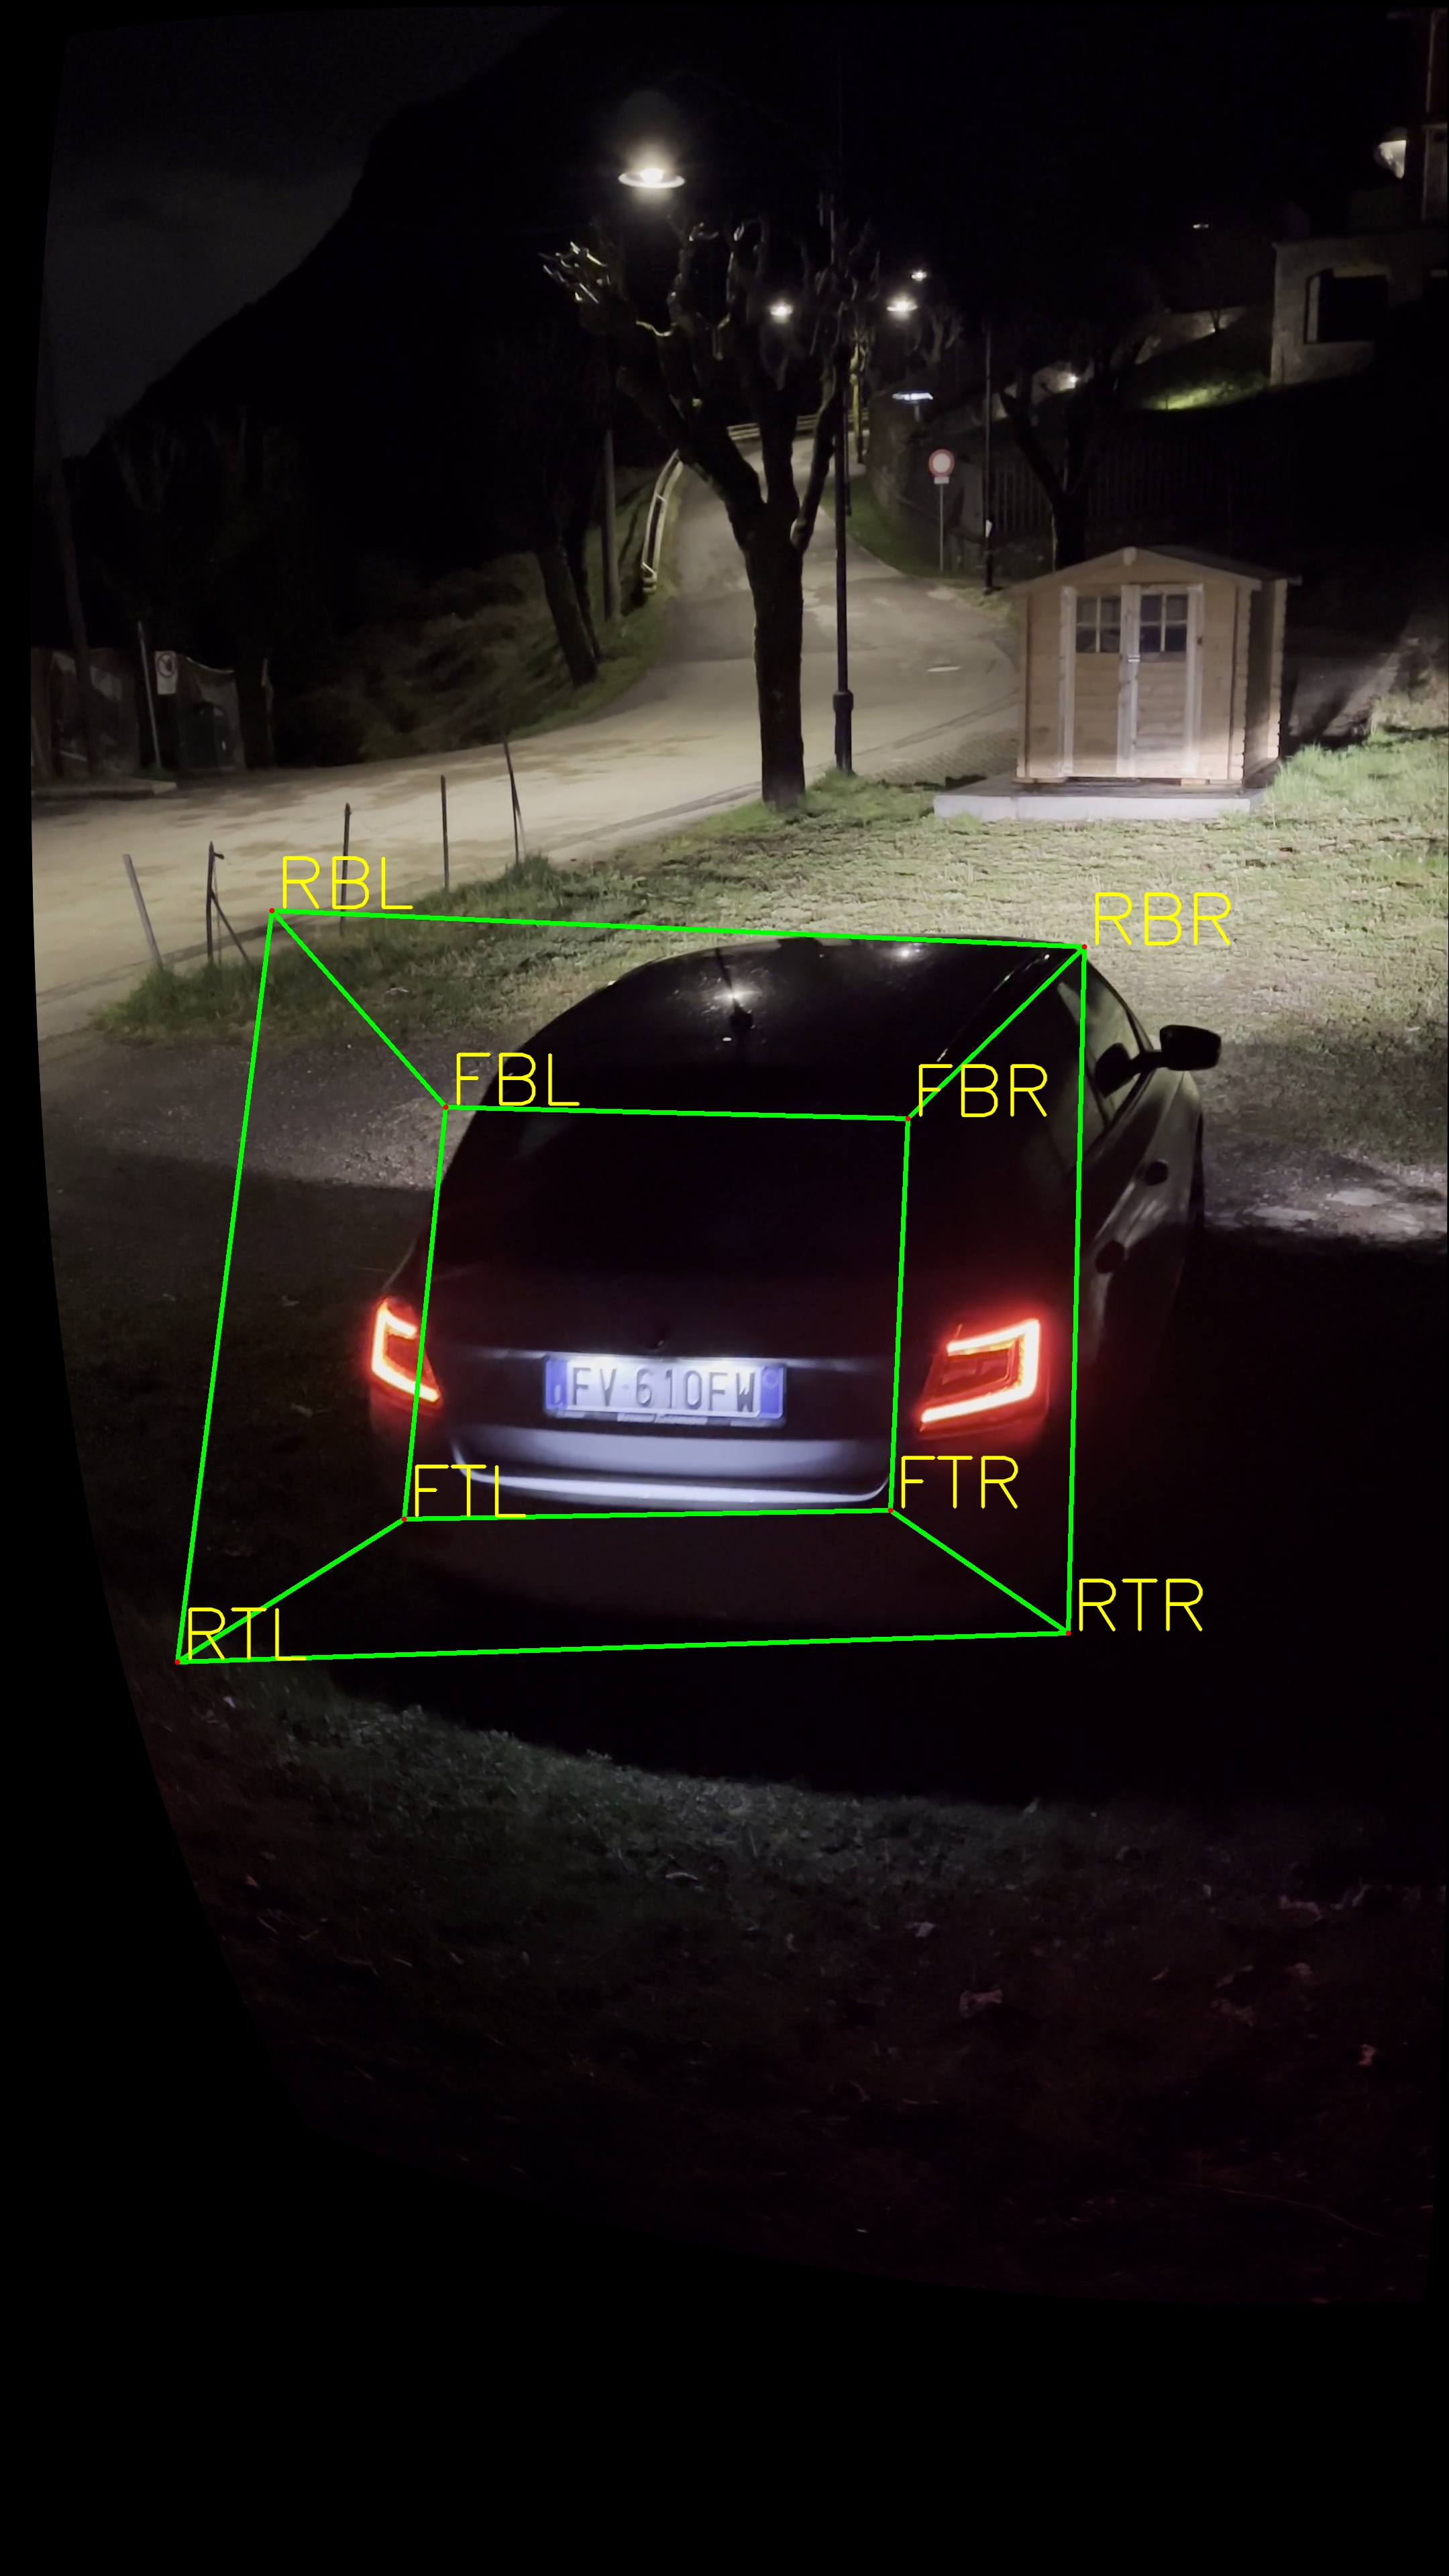
\includegraphics[width=0.20\textwidth]{Images/Conclusions/method1/1_frame4.jpg} &
        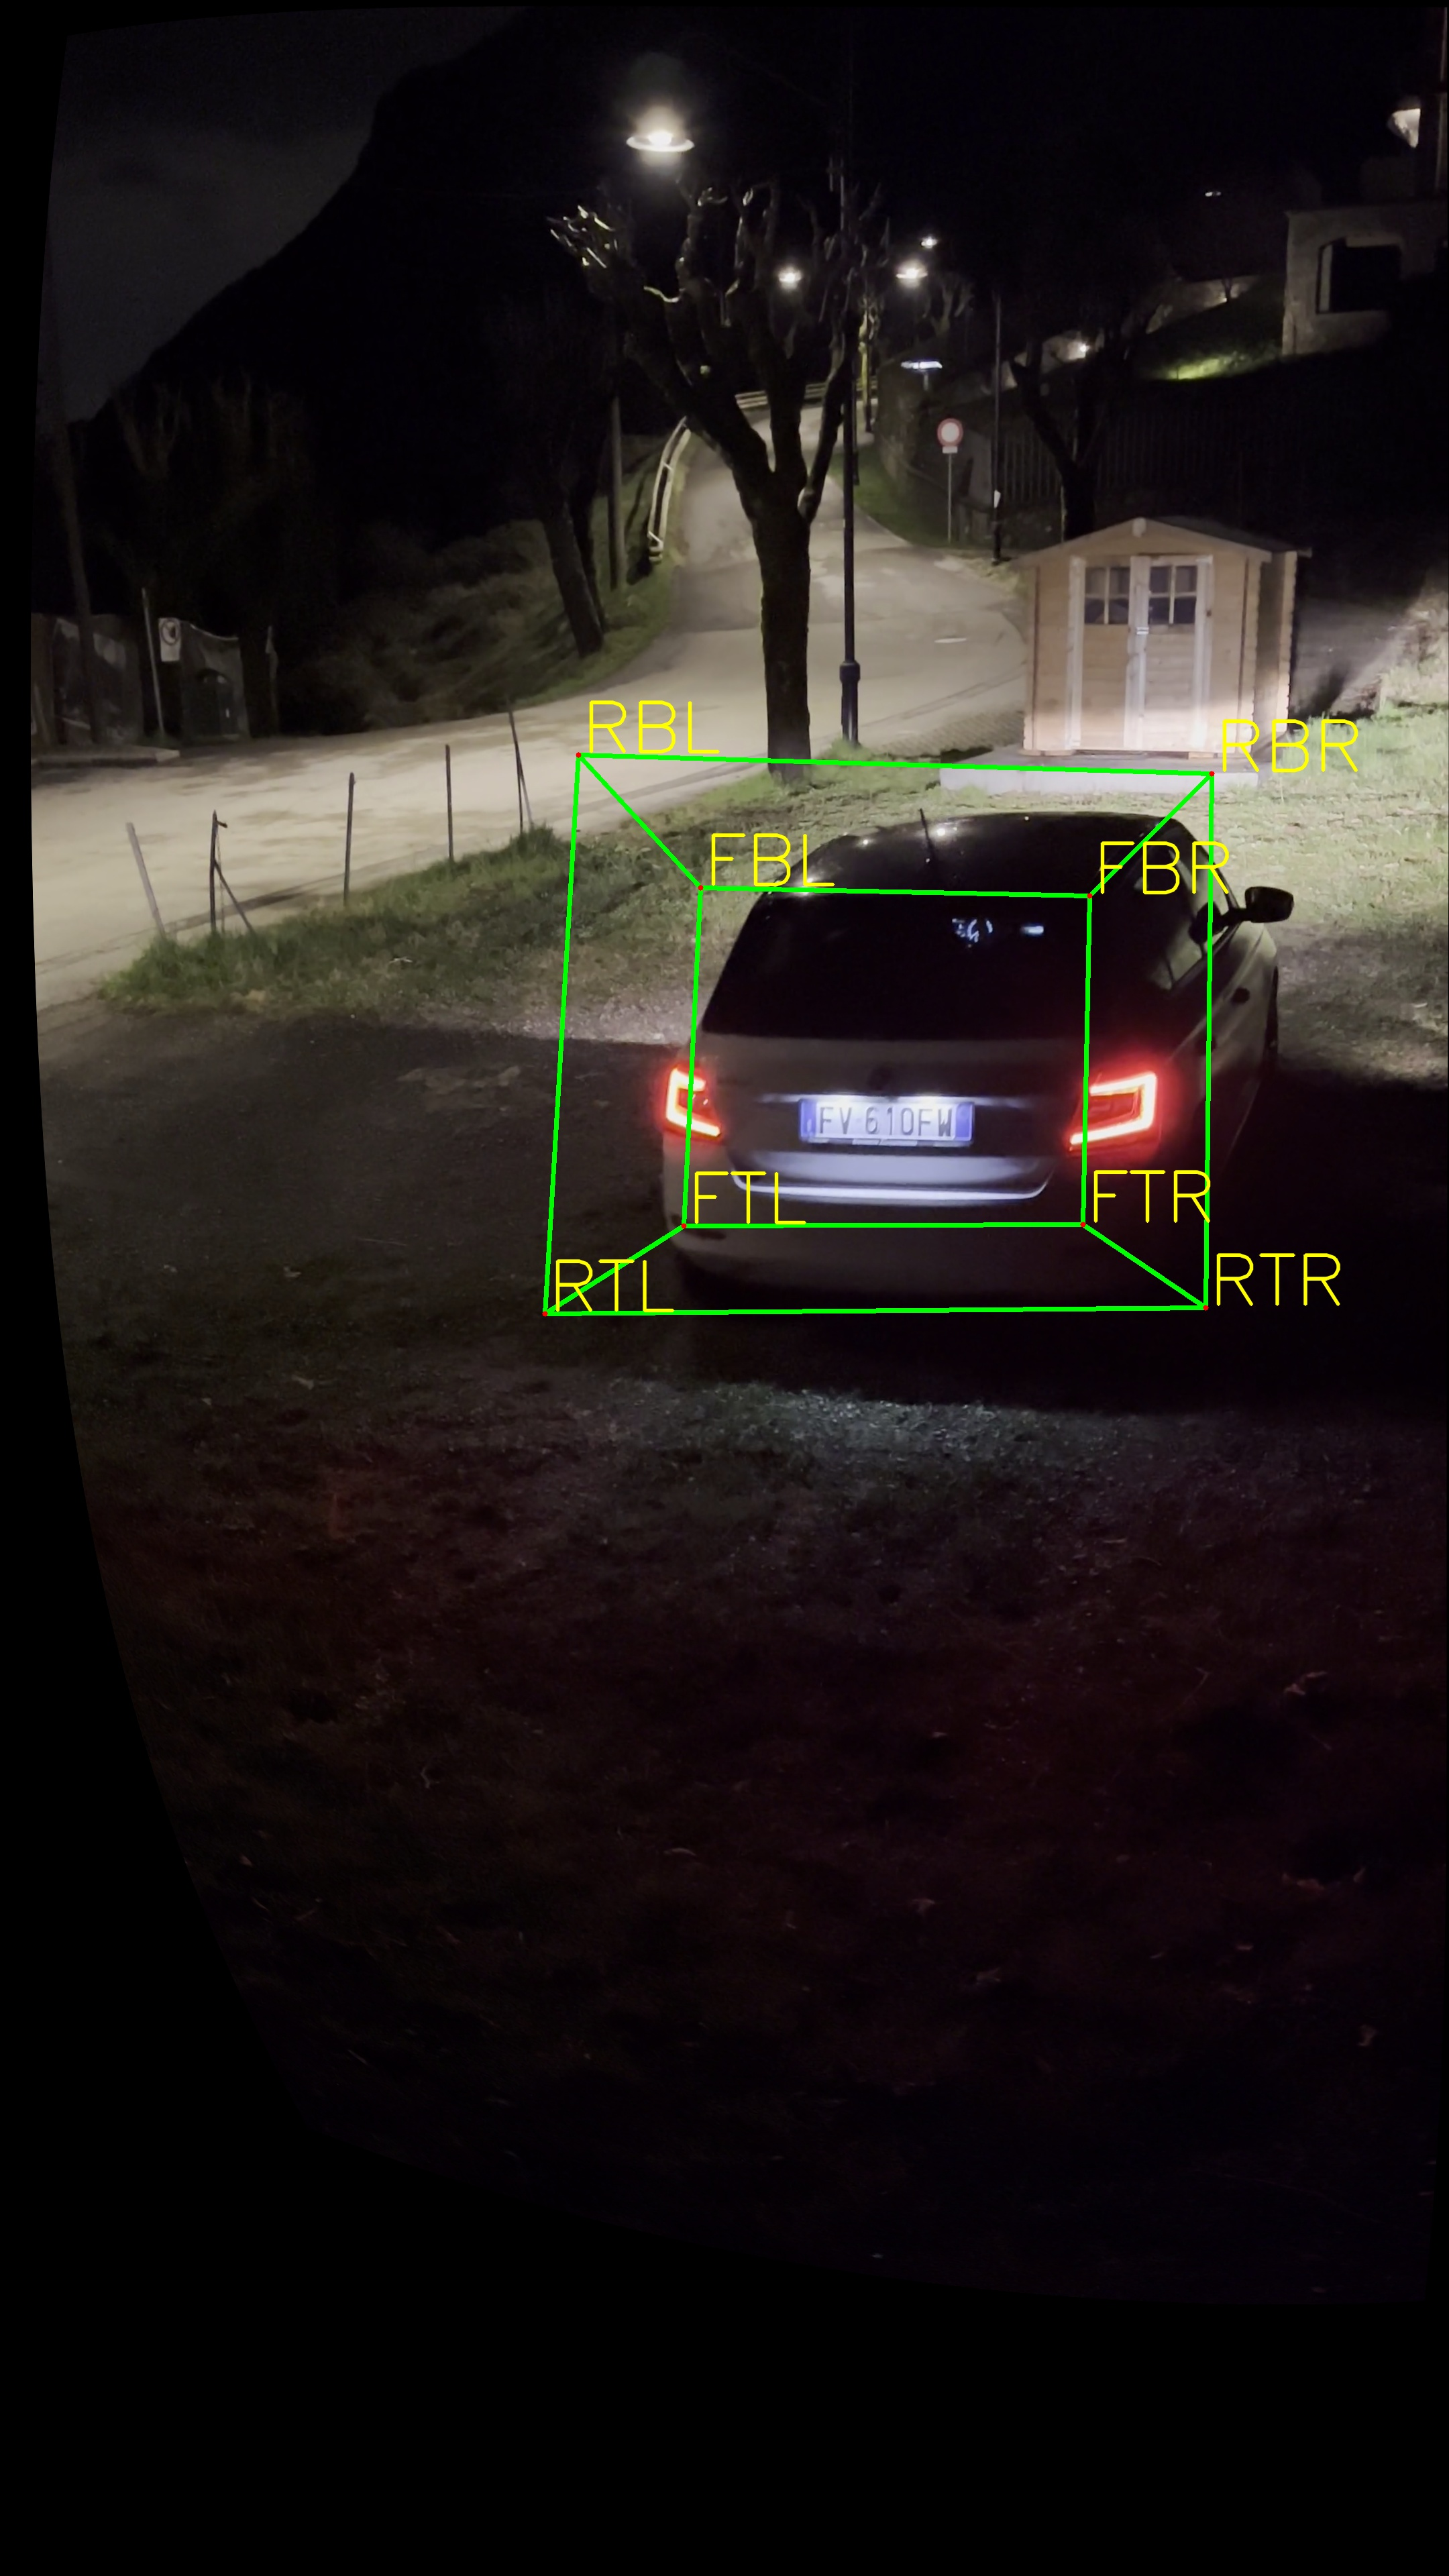
\includegraphics[width=0.20\textwidth]{Images/Conclusions/method1/1_frame8.jpg} &
        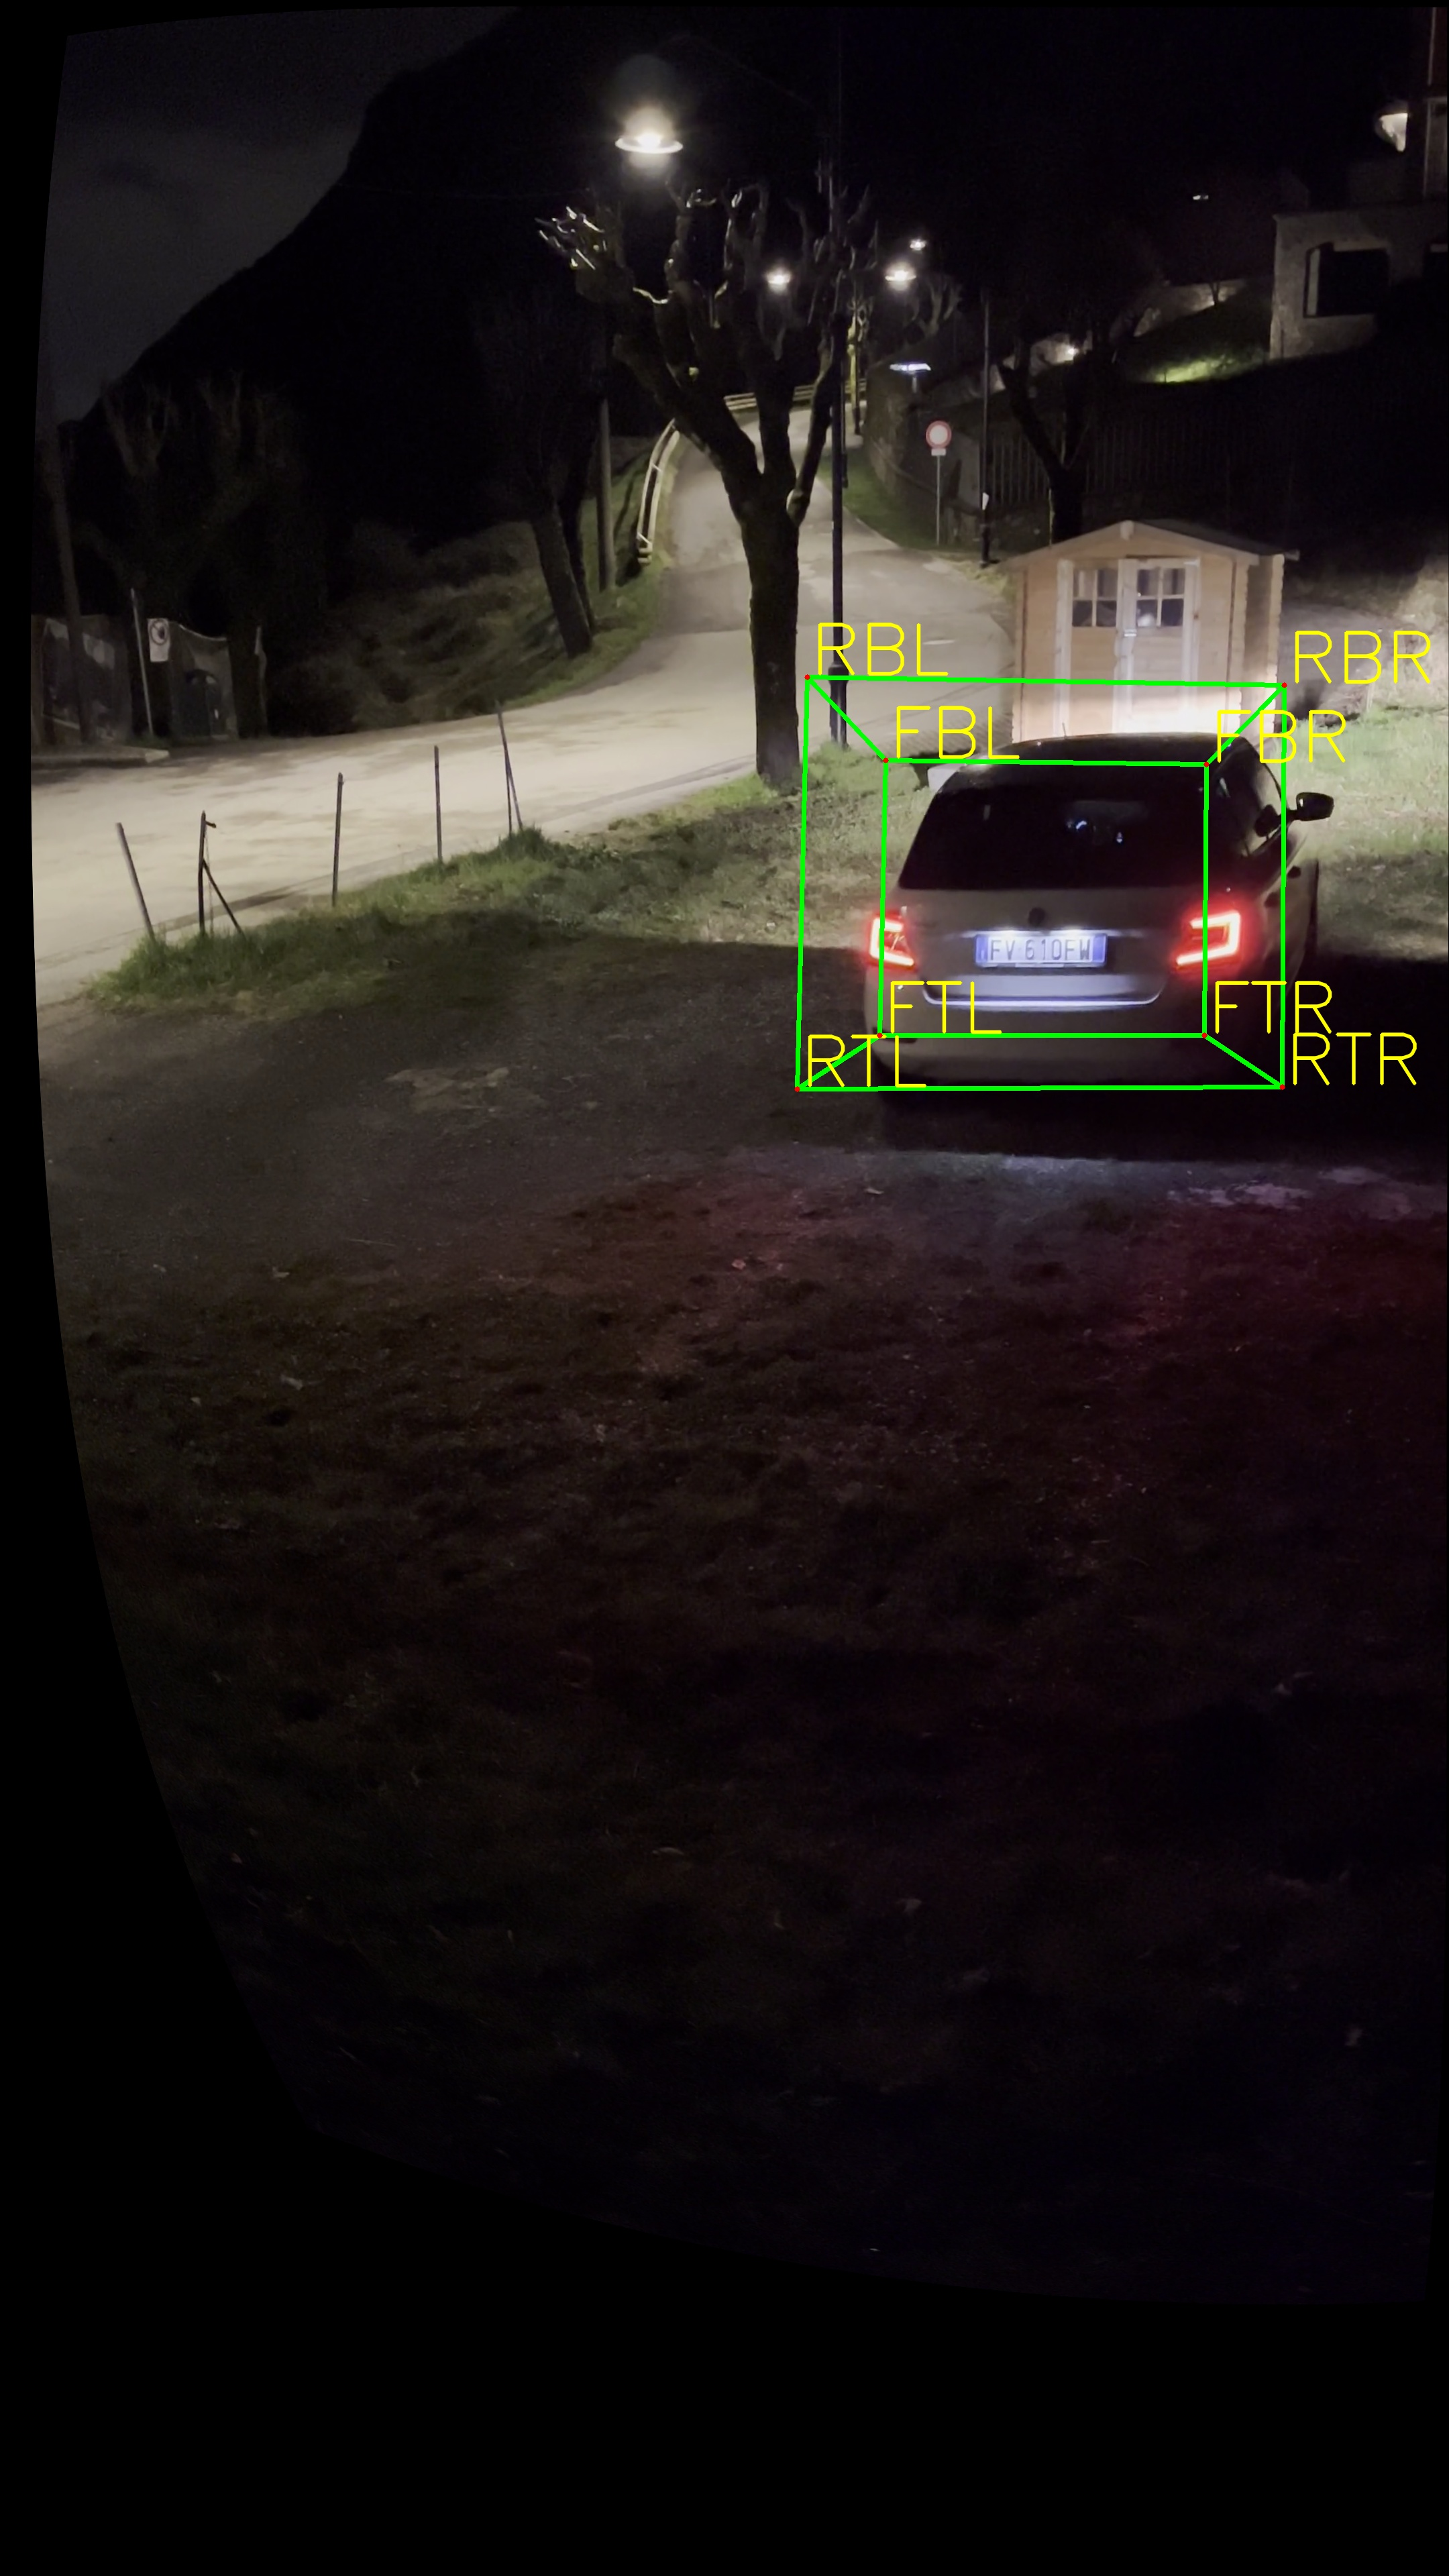
\includegraphics[width=0.20\textwidth]{Images/Conclusions/method1/1_frame12.jpg} &
        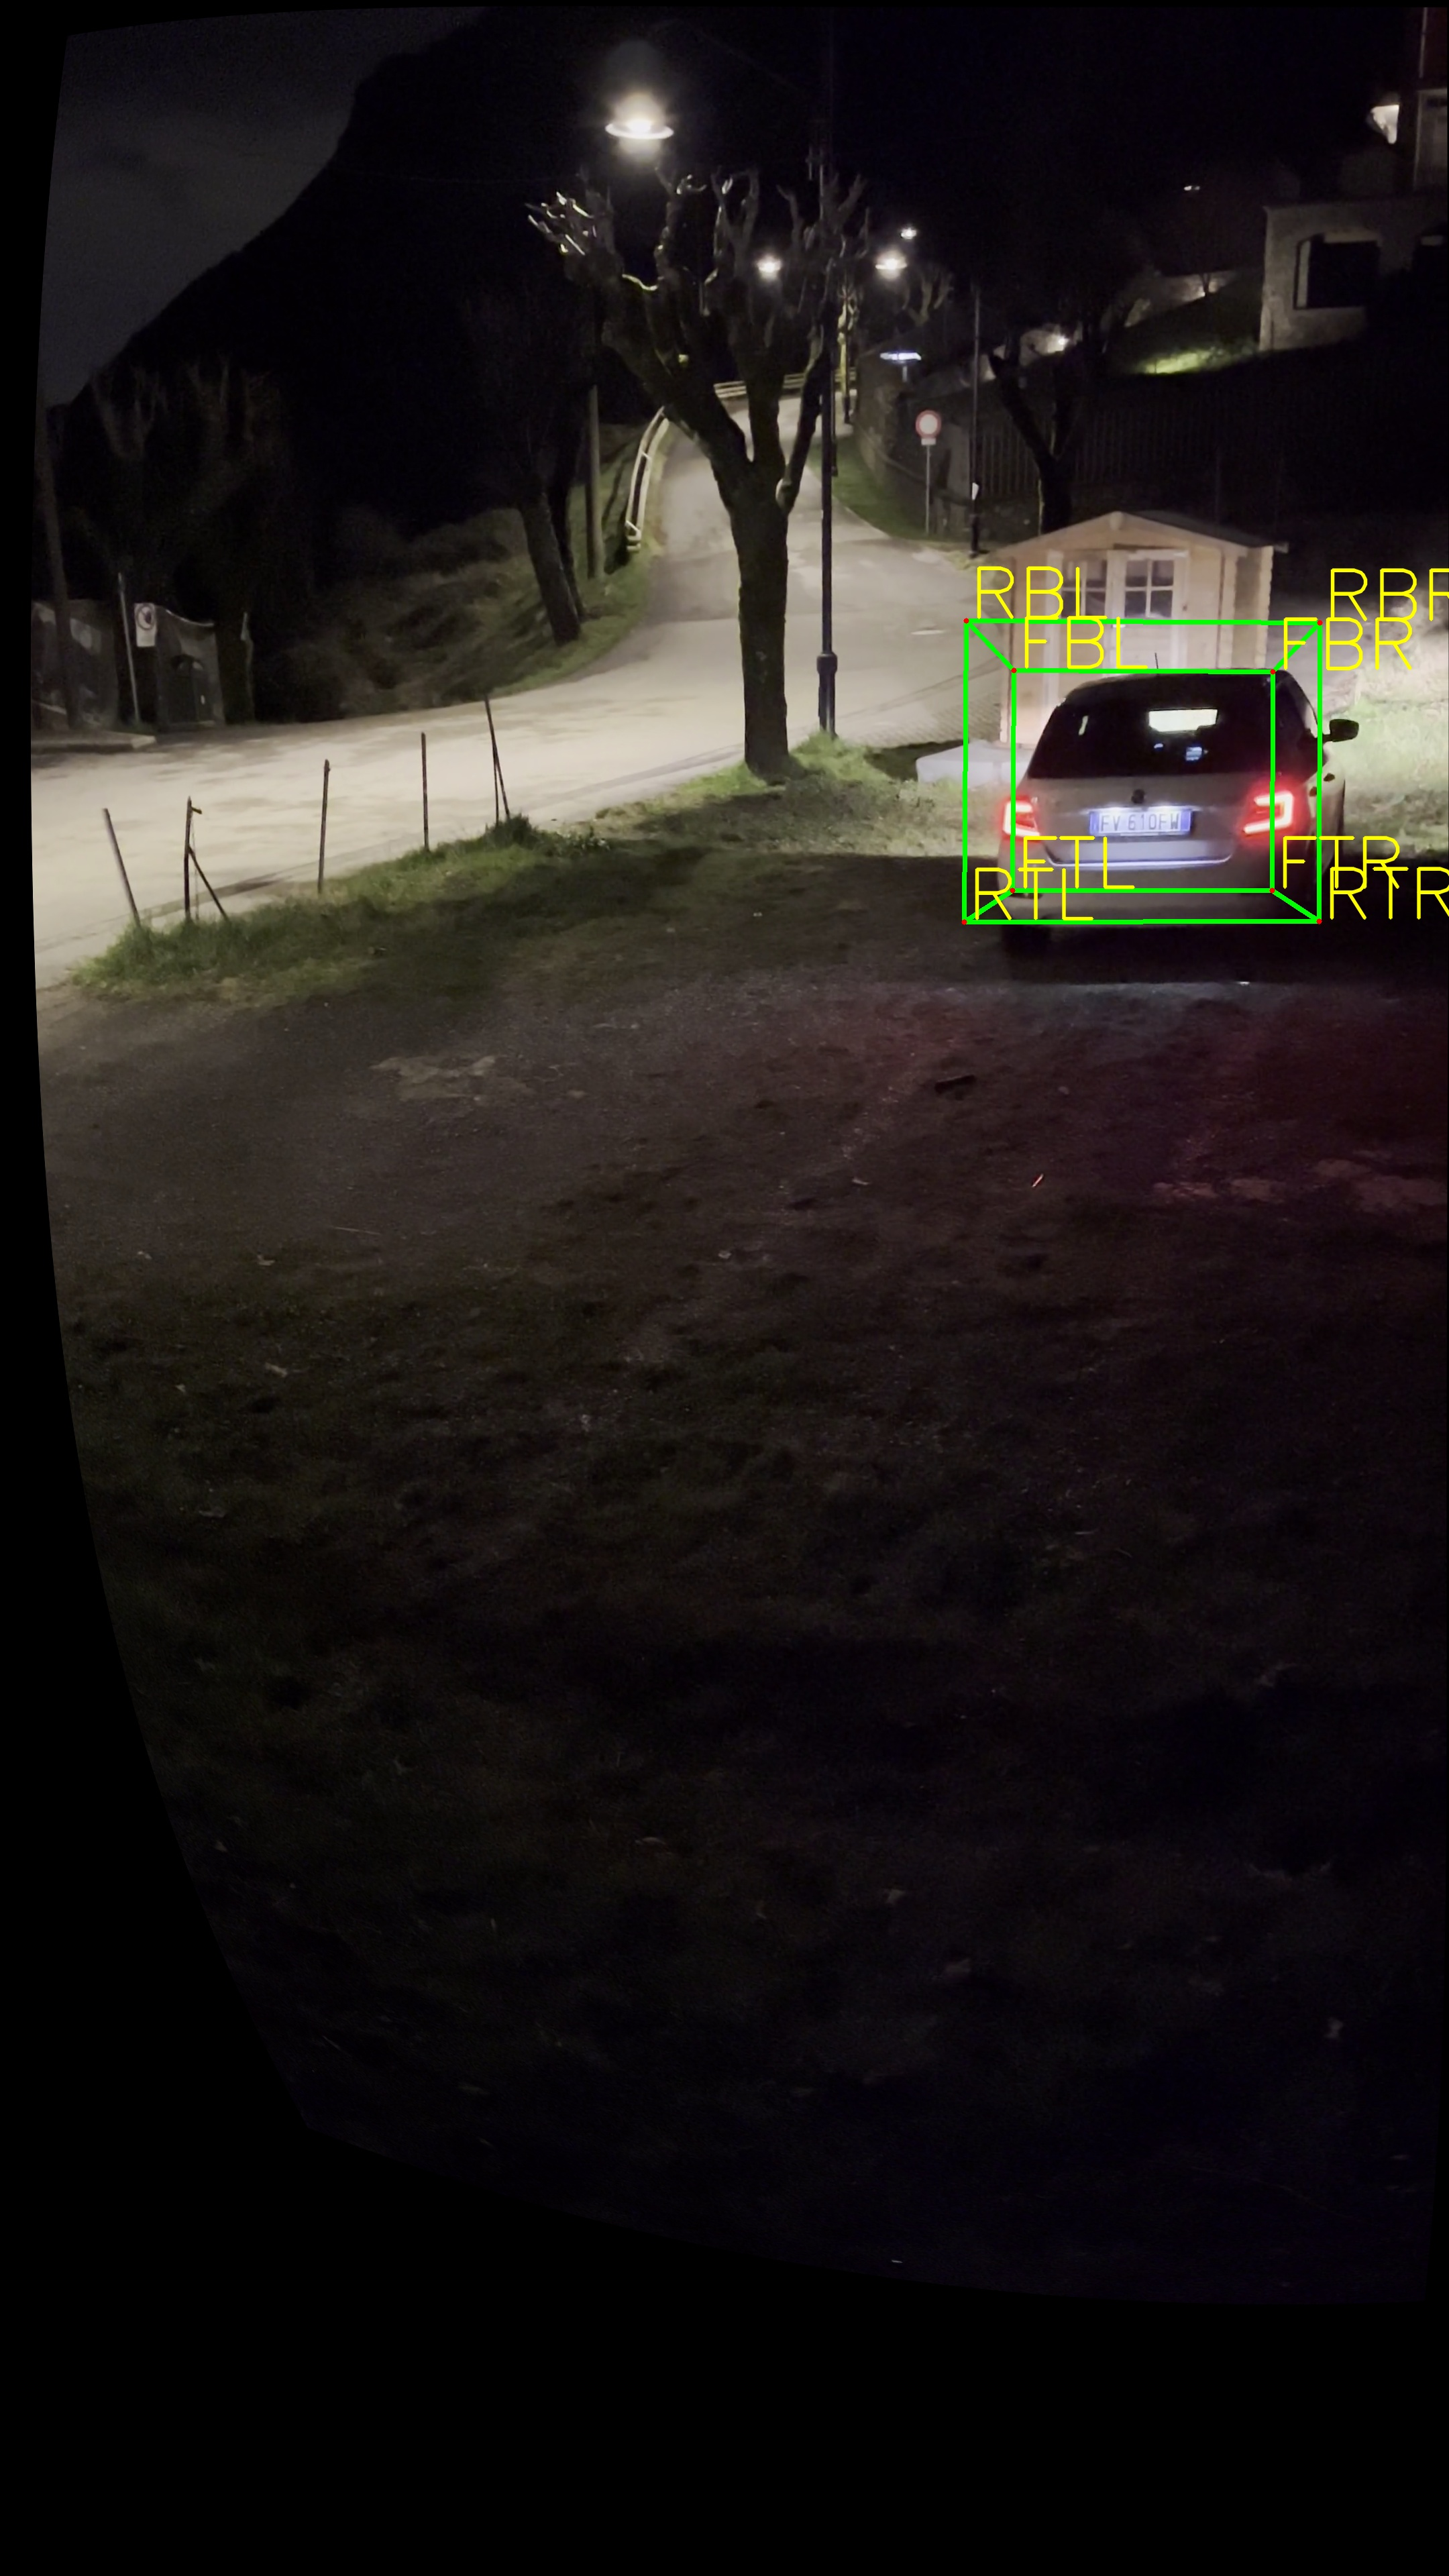
\includegraphics[width=0.20\textwidth]{Images/Conclusions/method1/1_frame16.jpg} \\[6pt]

        \raisebox{9\height}{\textbf{Method 2}} &
        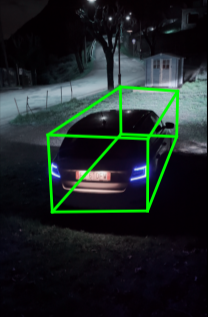
\includegraphics[width=0.20\textwidth]{Images/Conclusions/method2/2_frame4.png} &
        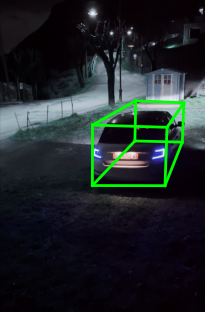
\includegraphics[width=0.20\textwidth]{Images/Conclusions/method2/2_frame8.png} &
        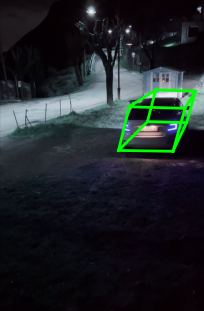
\includegraphics[width=0.20\textwidth]{Images/Conclusions/method2/2_frame12.png} &
        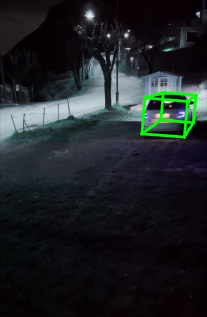
\includegraphics[width=0.20\textwidth]{Images/Conclusions/method2/2_frame16.png} \\[6pt]

        \raisebox{9\height}{\textbf{Method 3}} &
        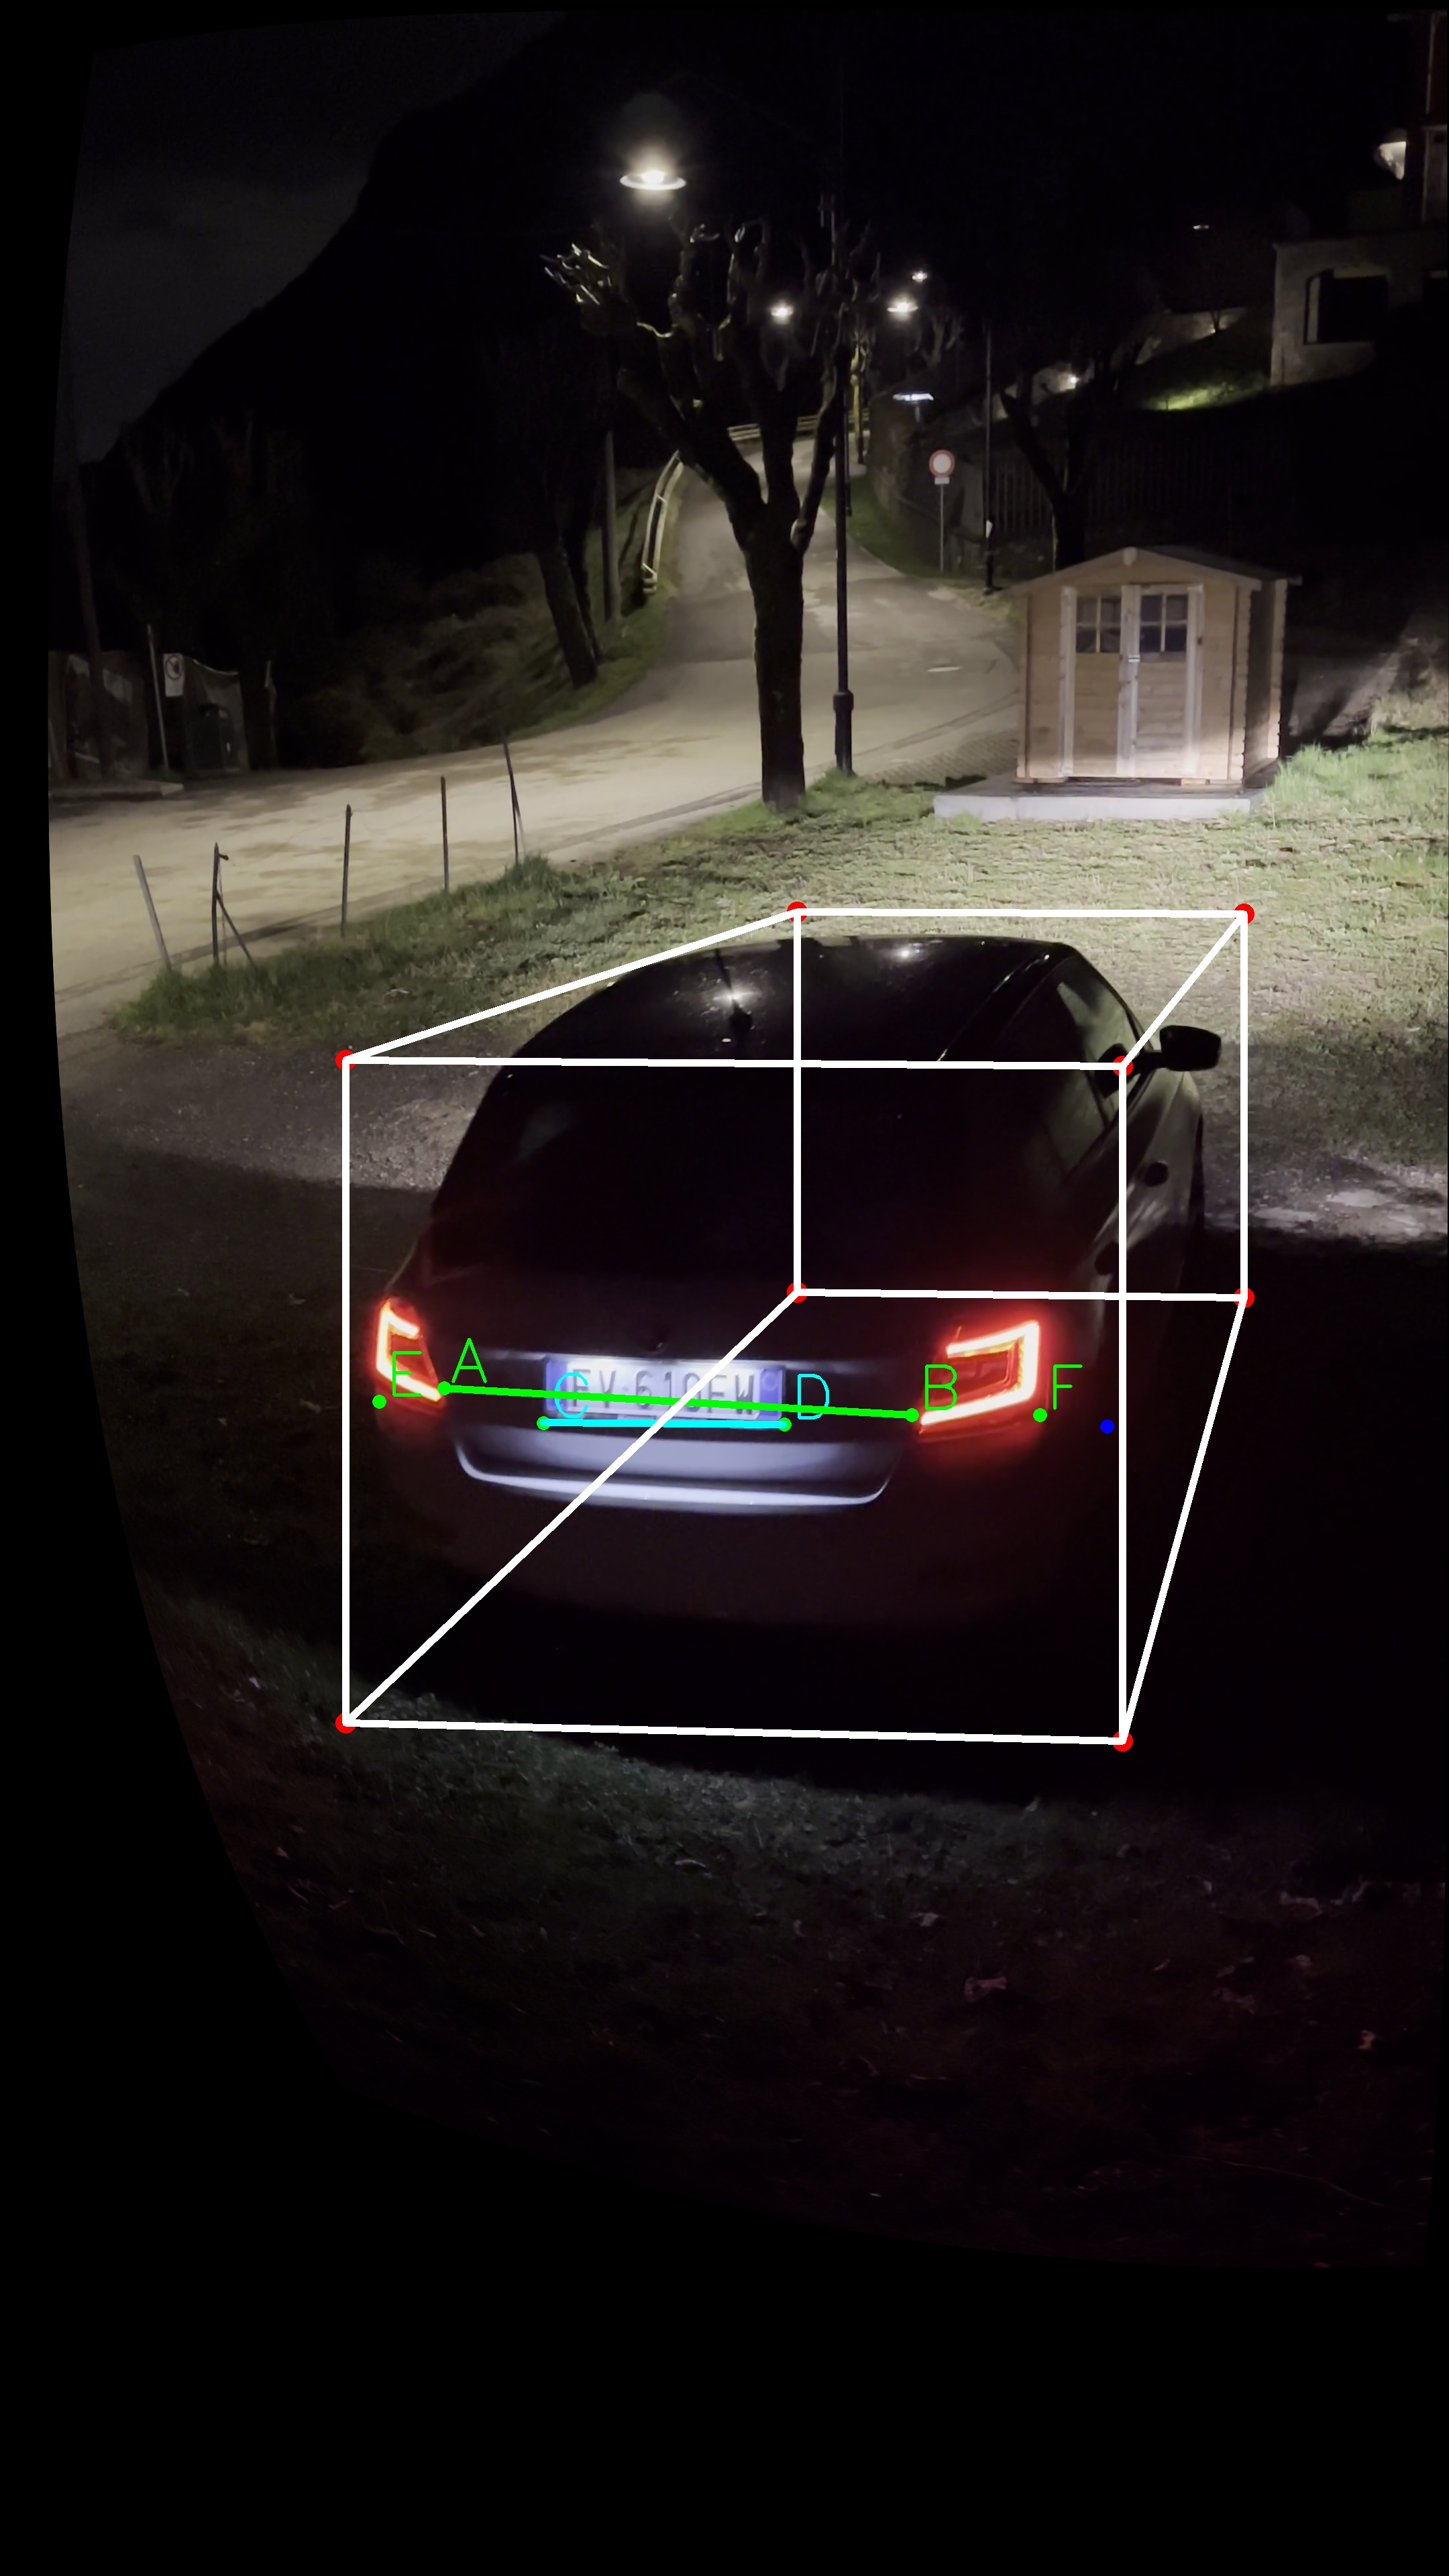
\includegraphics[width=0.20\textwidth]{Images/Conclusions/method3/3_frame4.jpg} &
        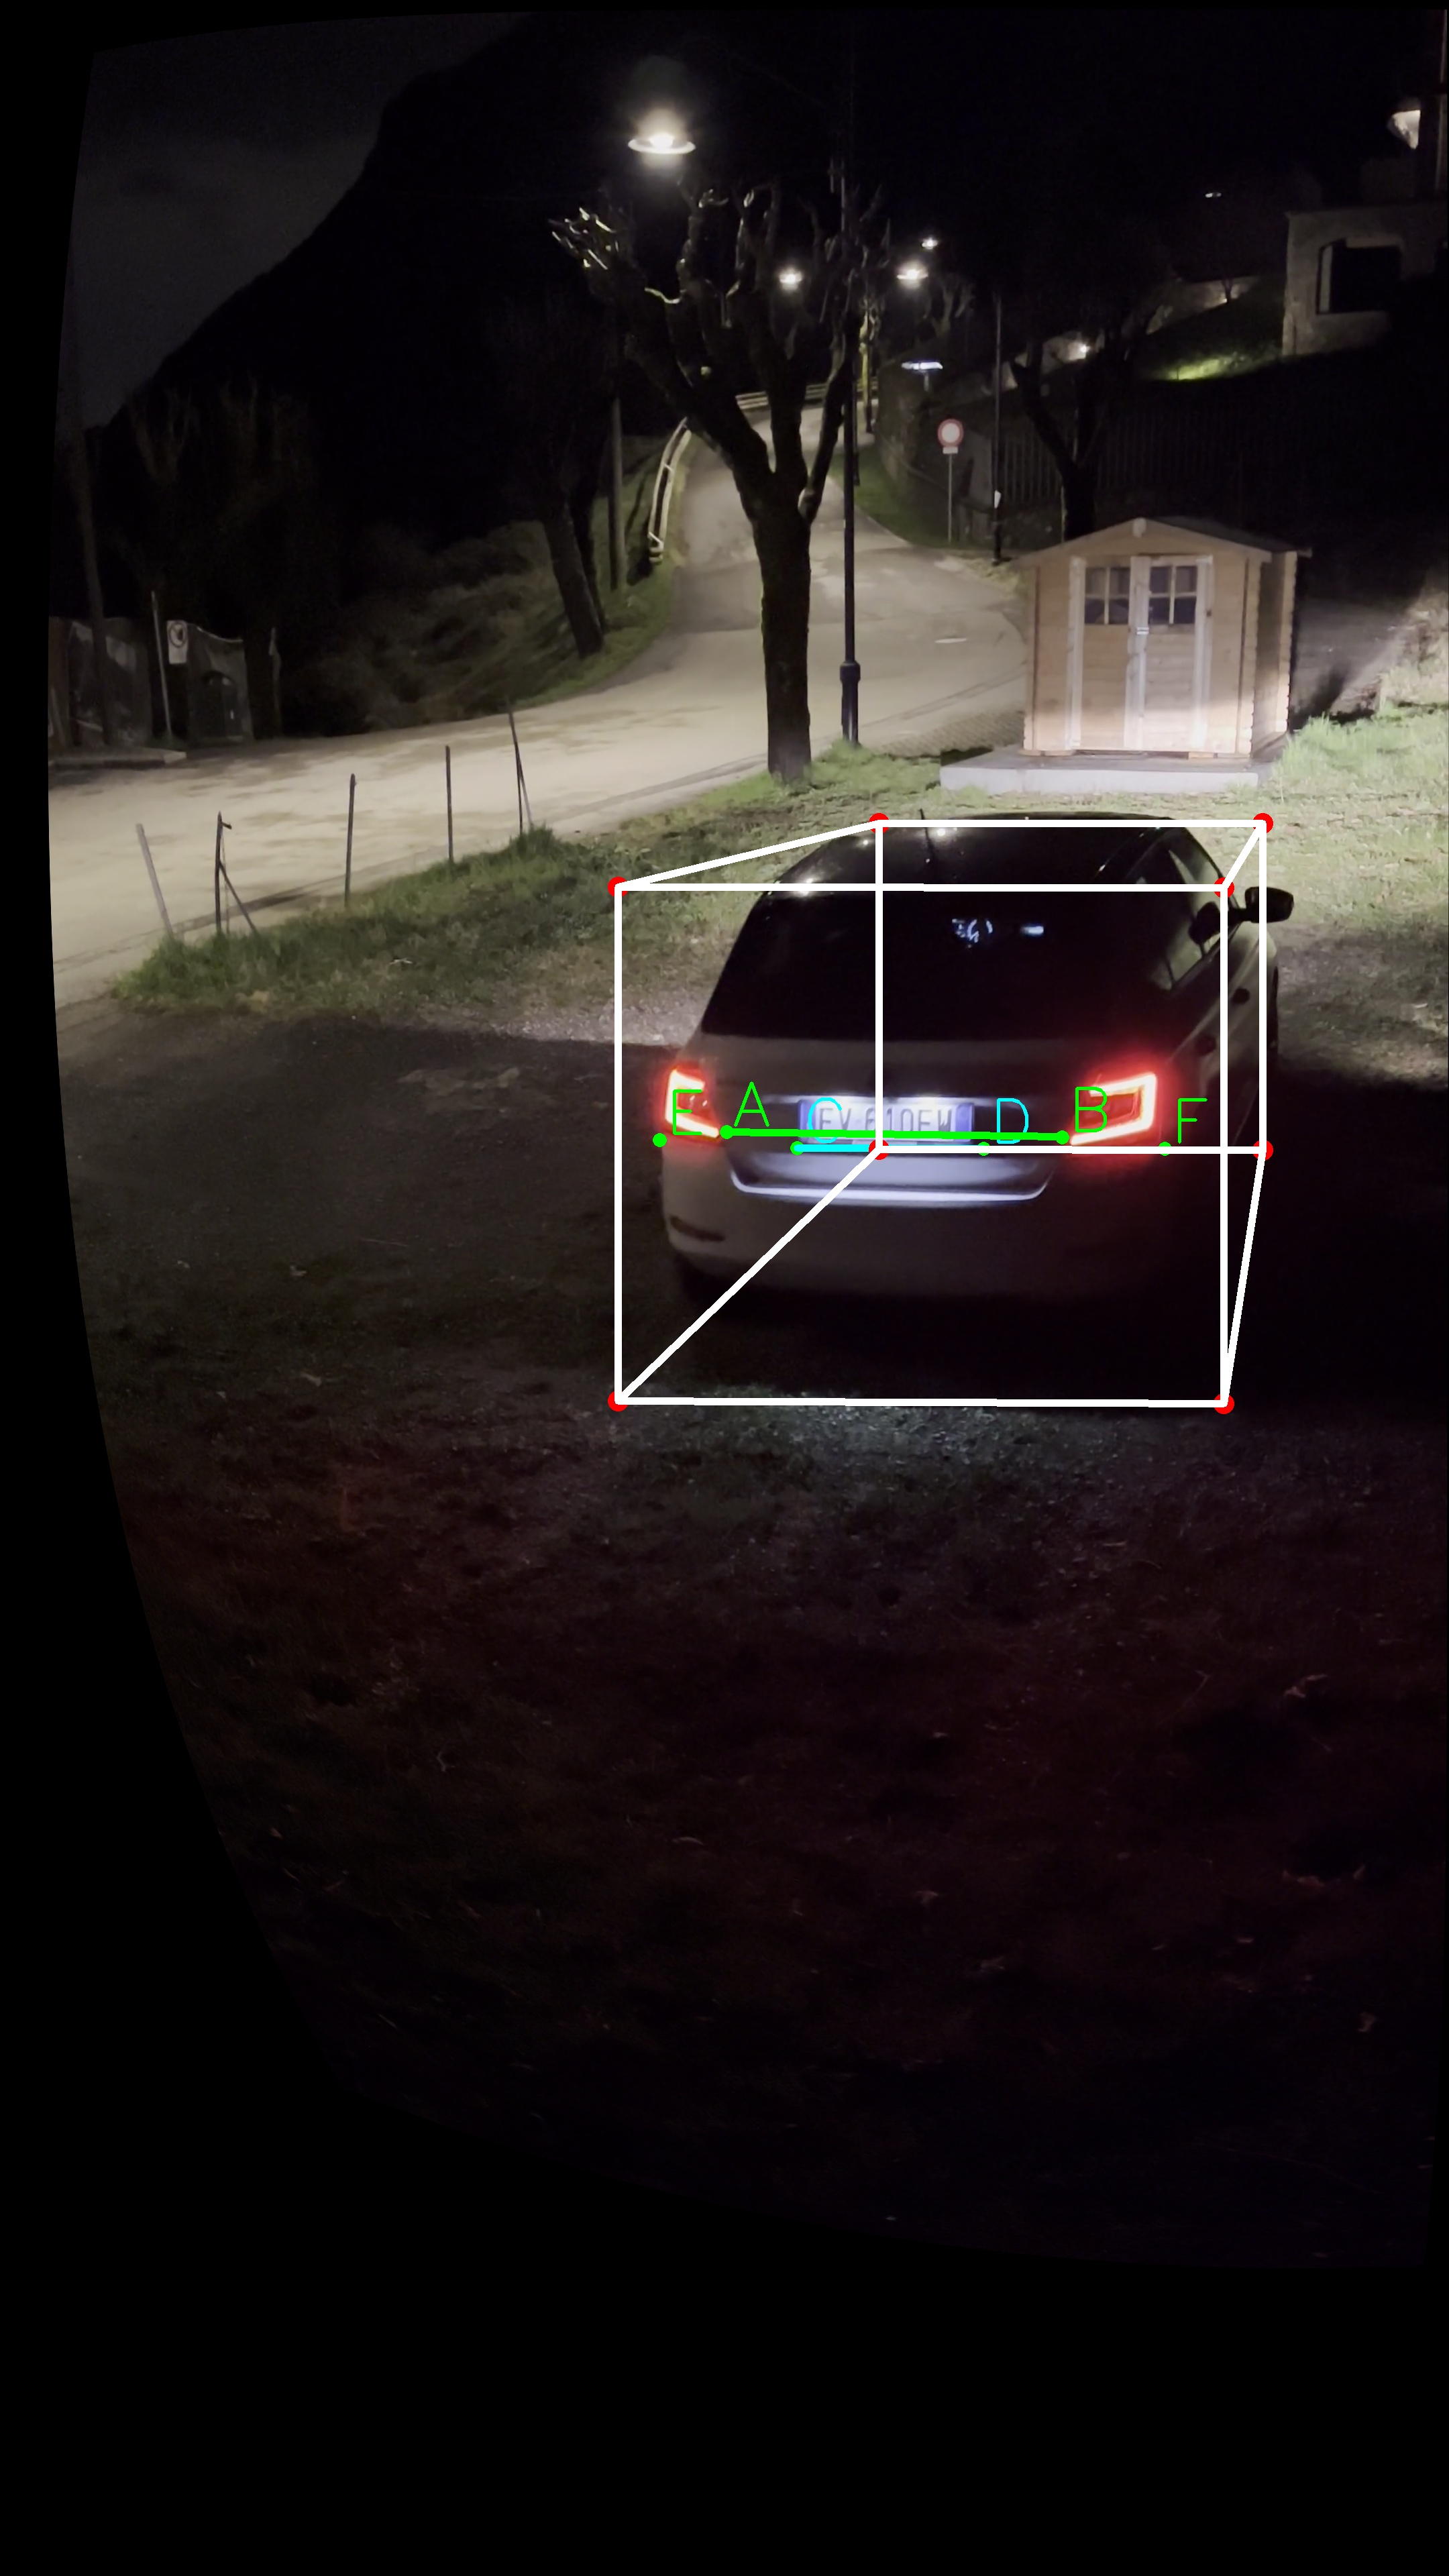
\includegraphics[width=0.20\textwidth]{Images/Conclusions/method3/3_frame8.jpg} &
        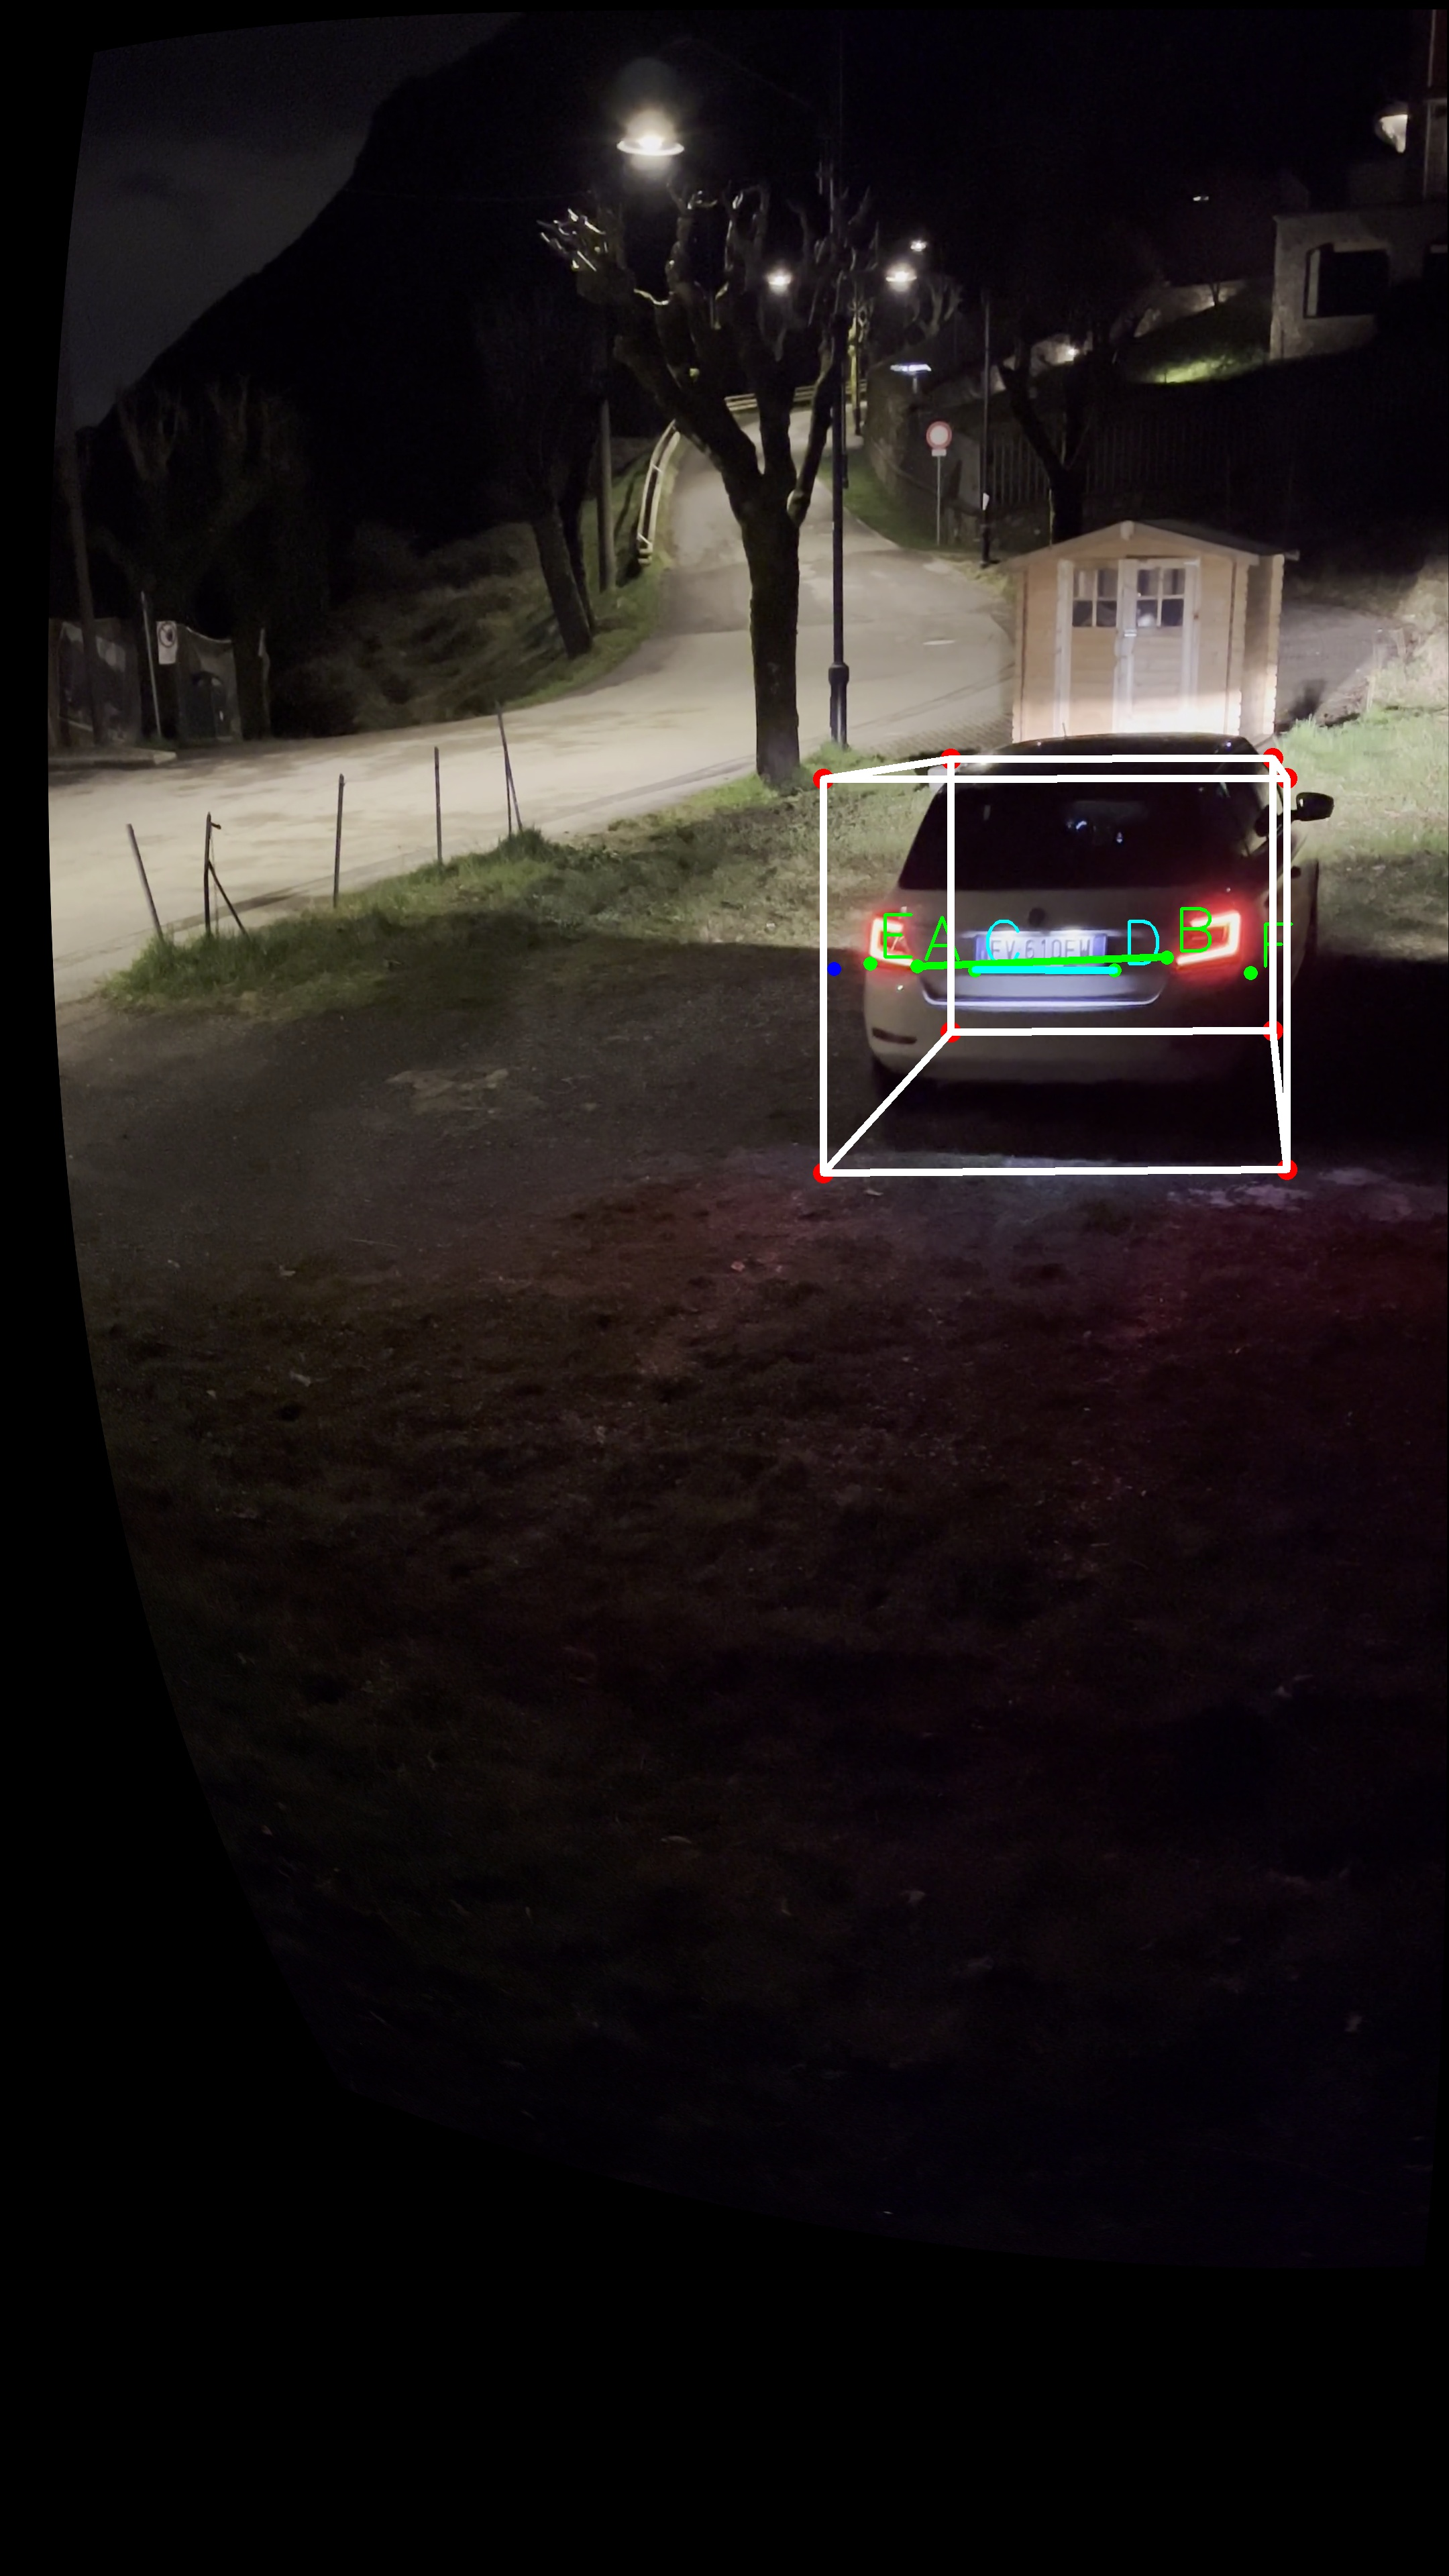
\includegraphics[width=0.20\textwidth]{Images/Conclusions/method3/3_frame12.jpg} &
        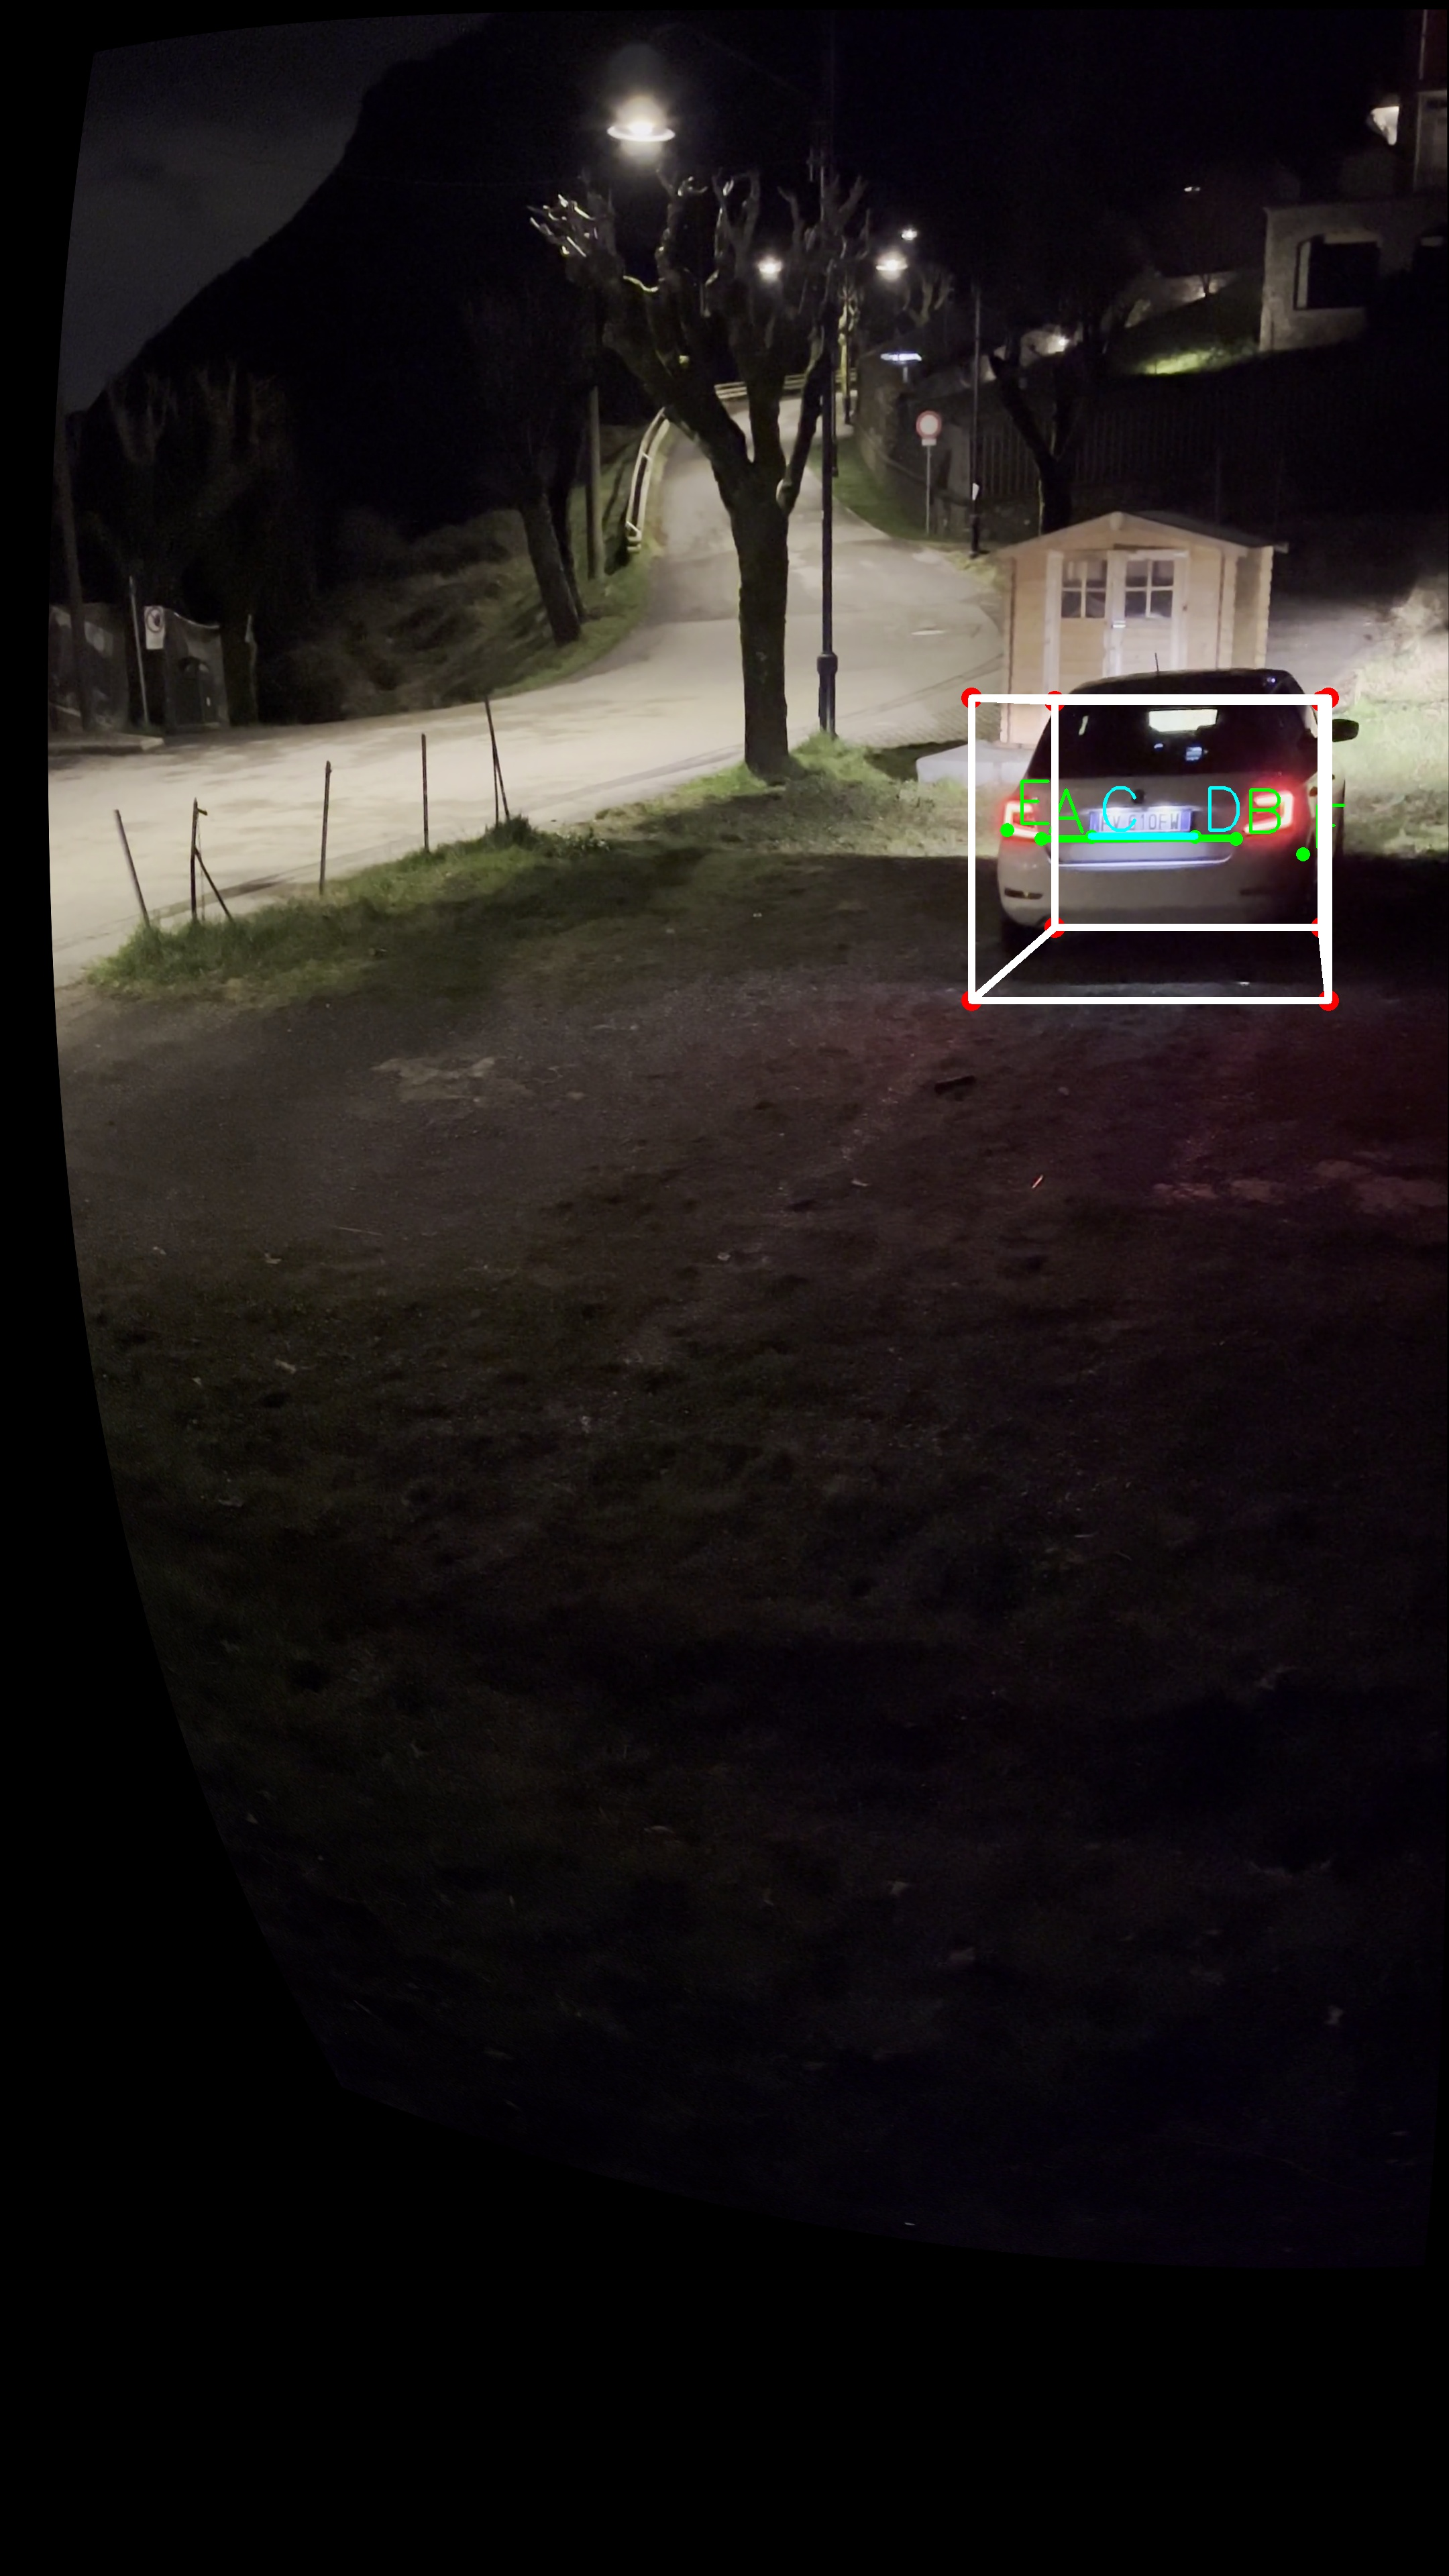
\includegraphics[width=0.20\textwidth]{Images/Conclusions/method3/3_frame16.jpg} \\[6pt]

        \raisebox{9\height}{\textbf{Method 4}} &
        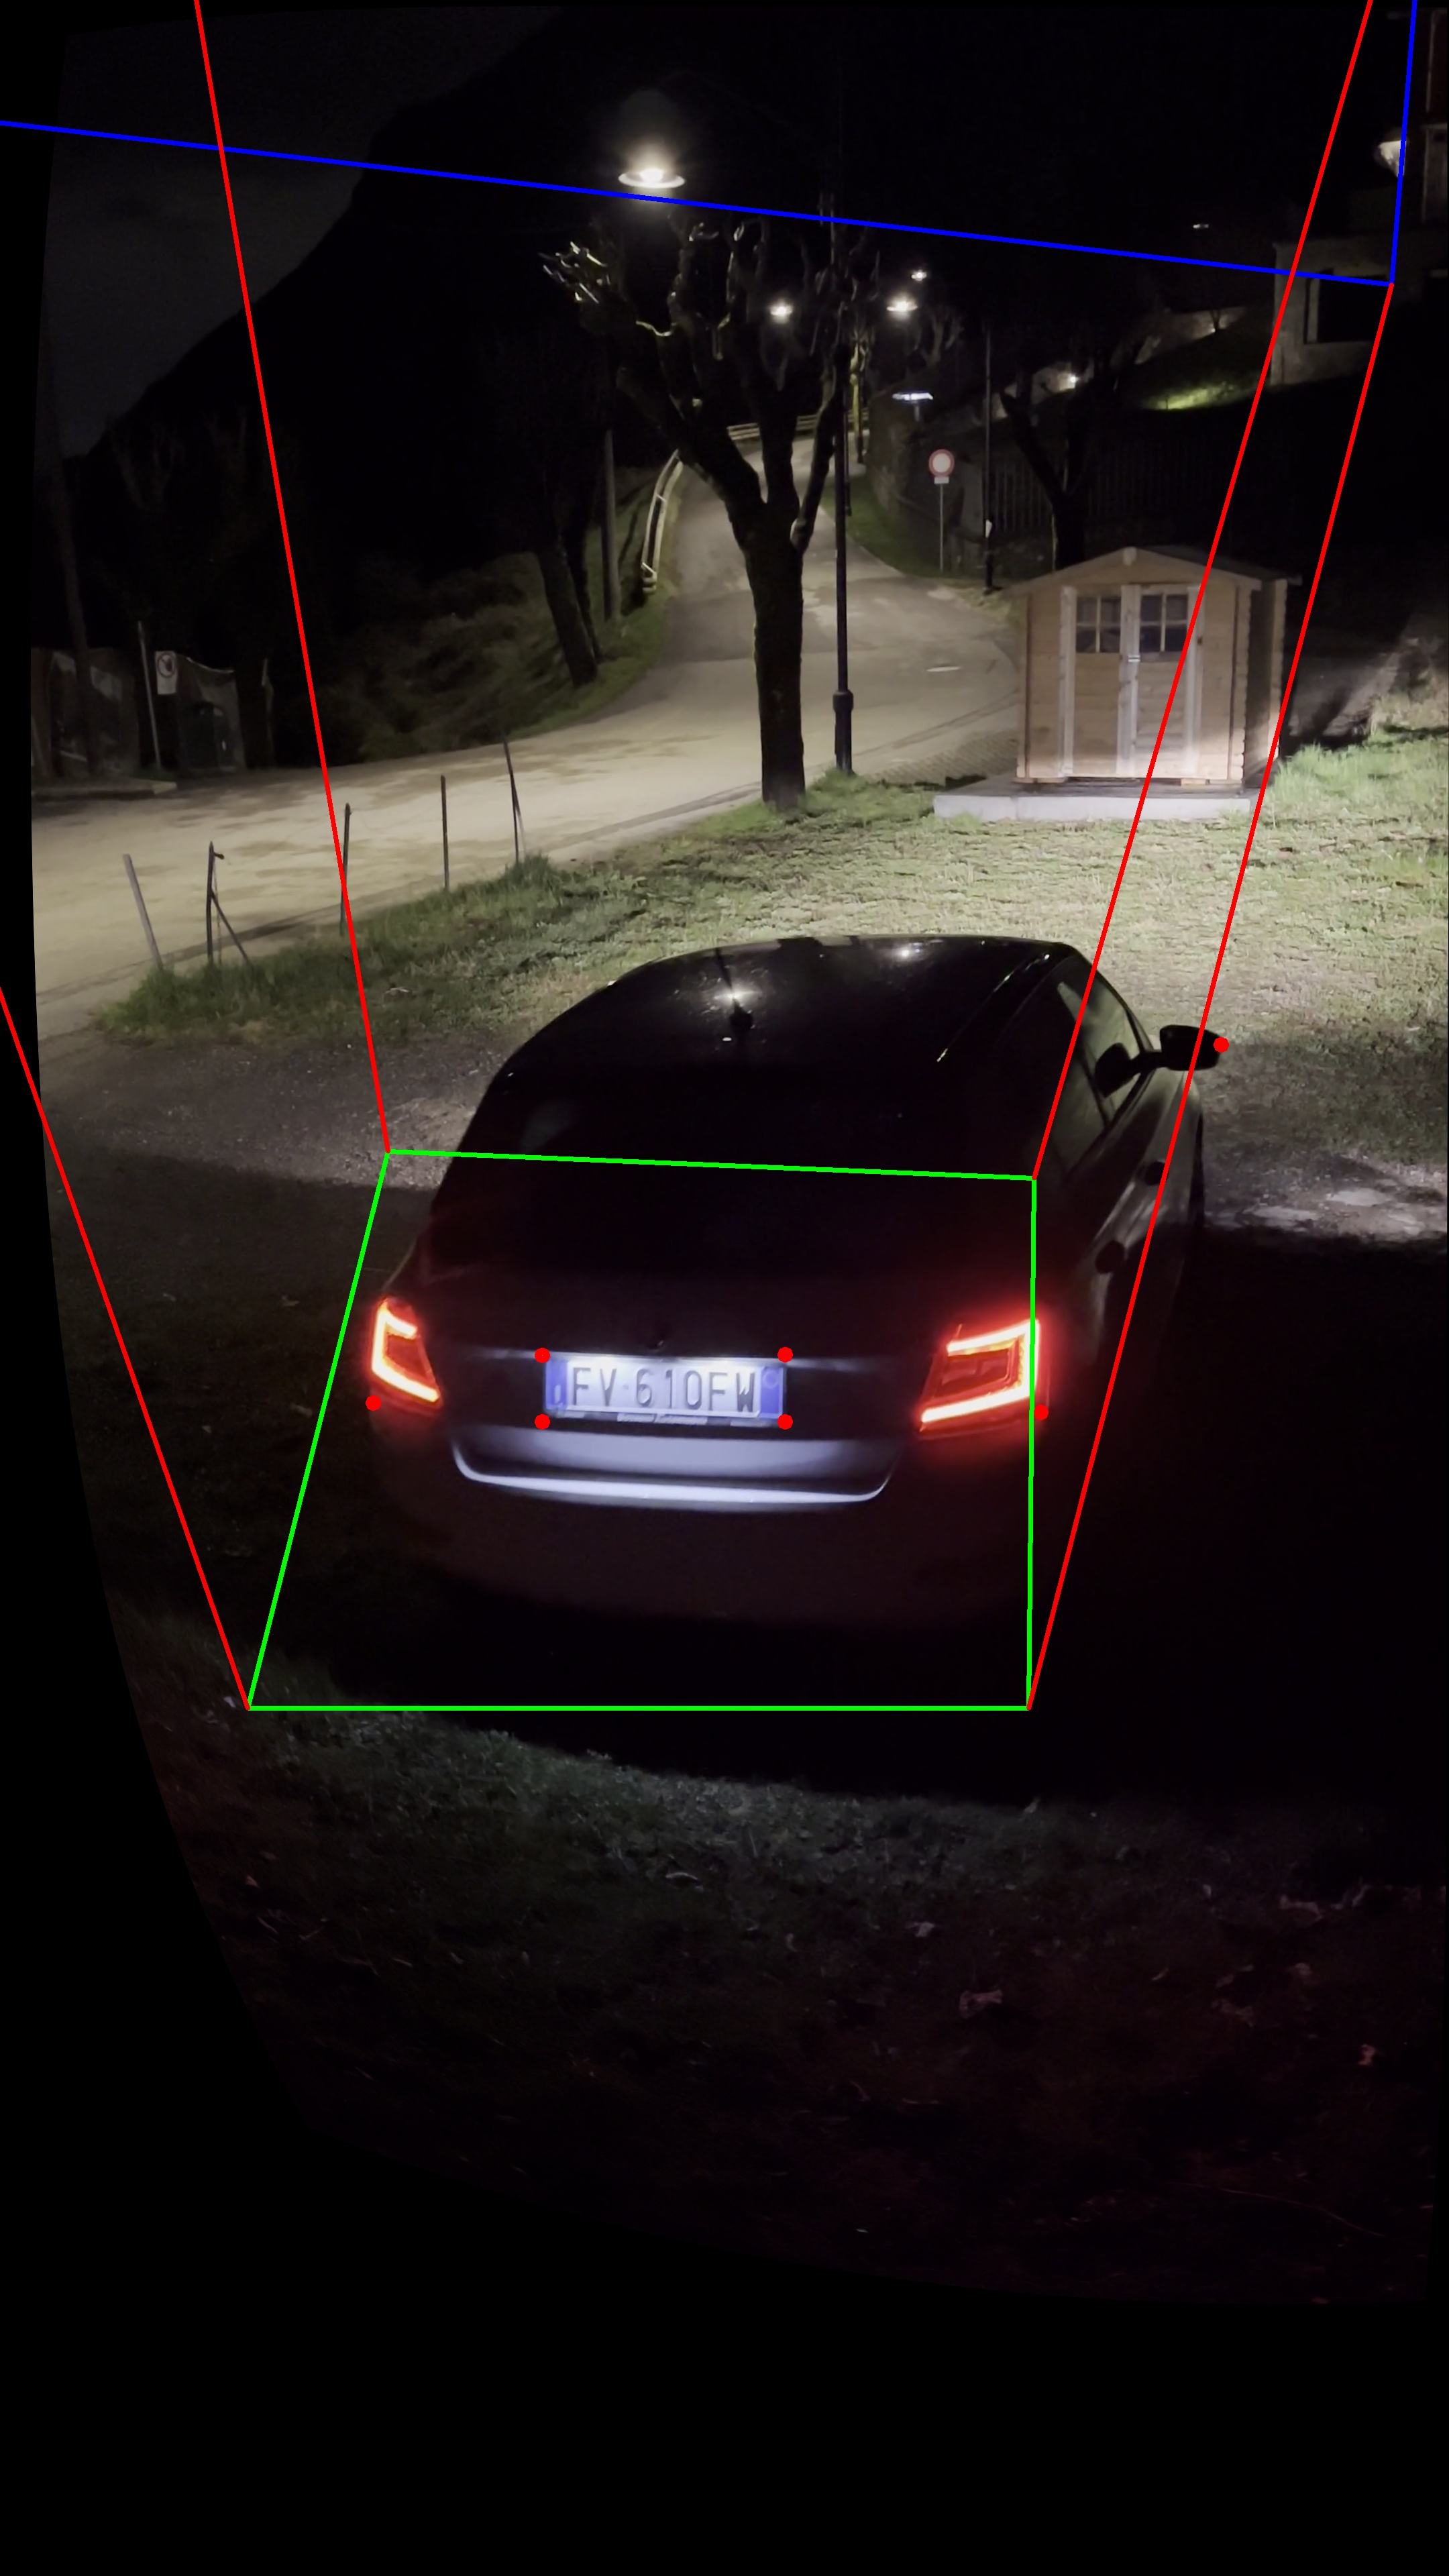
\includegraphics[width=0.20\textwidth]{Images/Conclusions/method4/4_frame4.jpg} &
        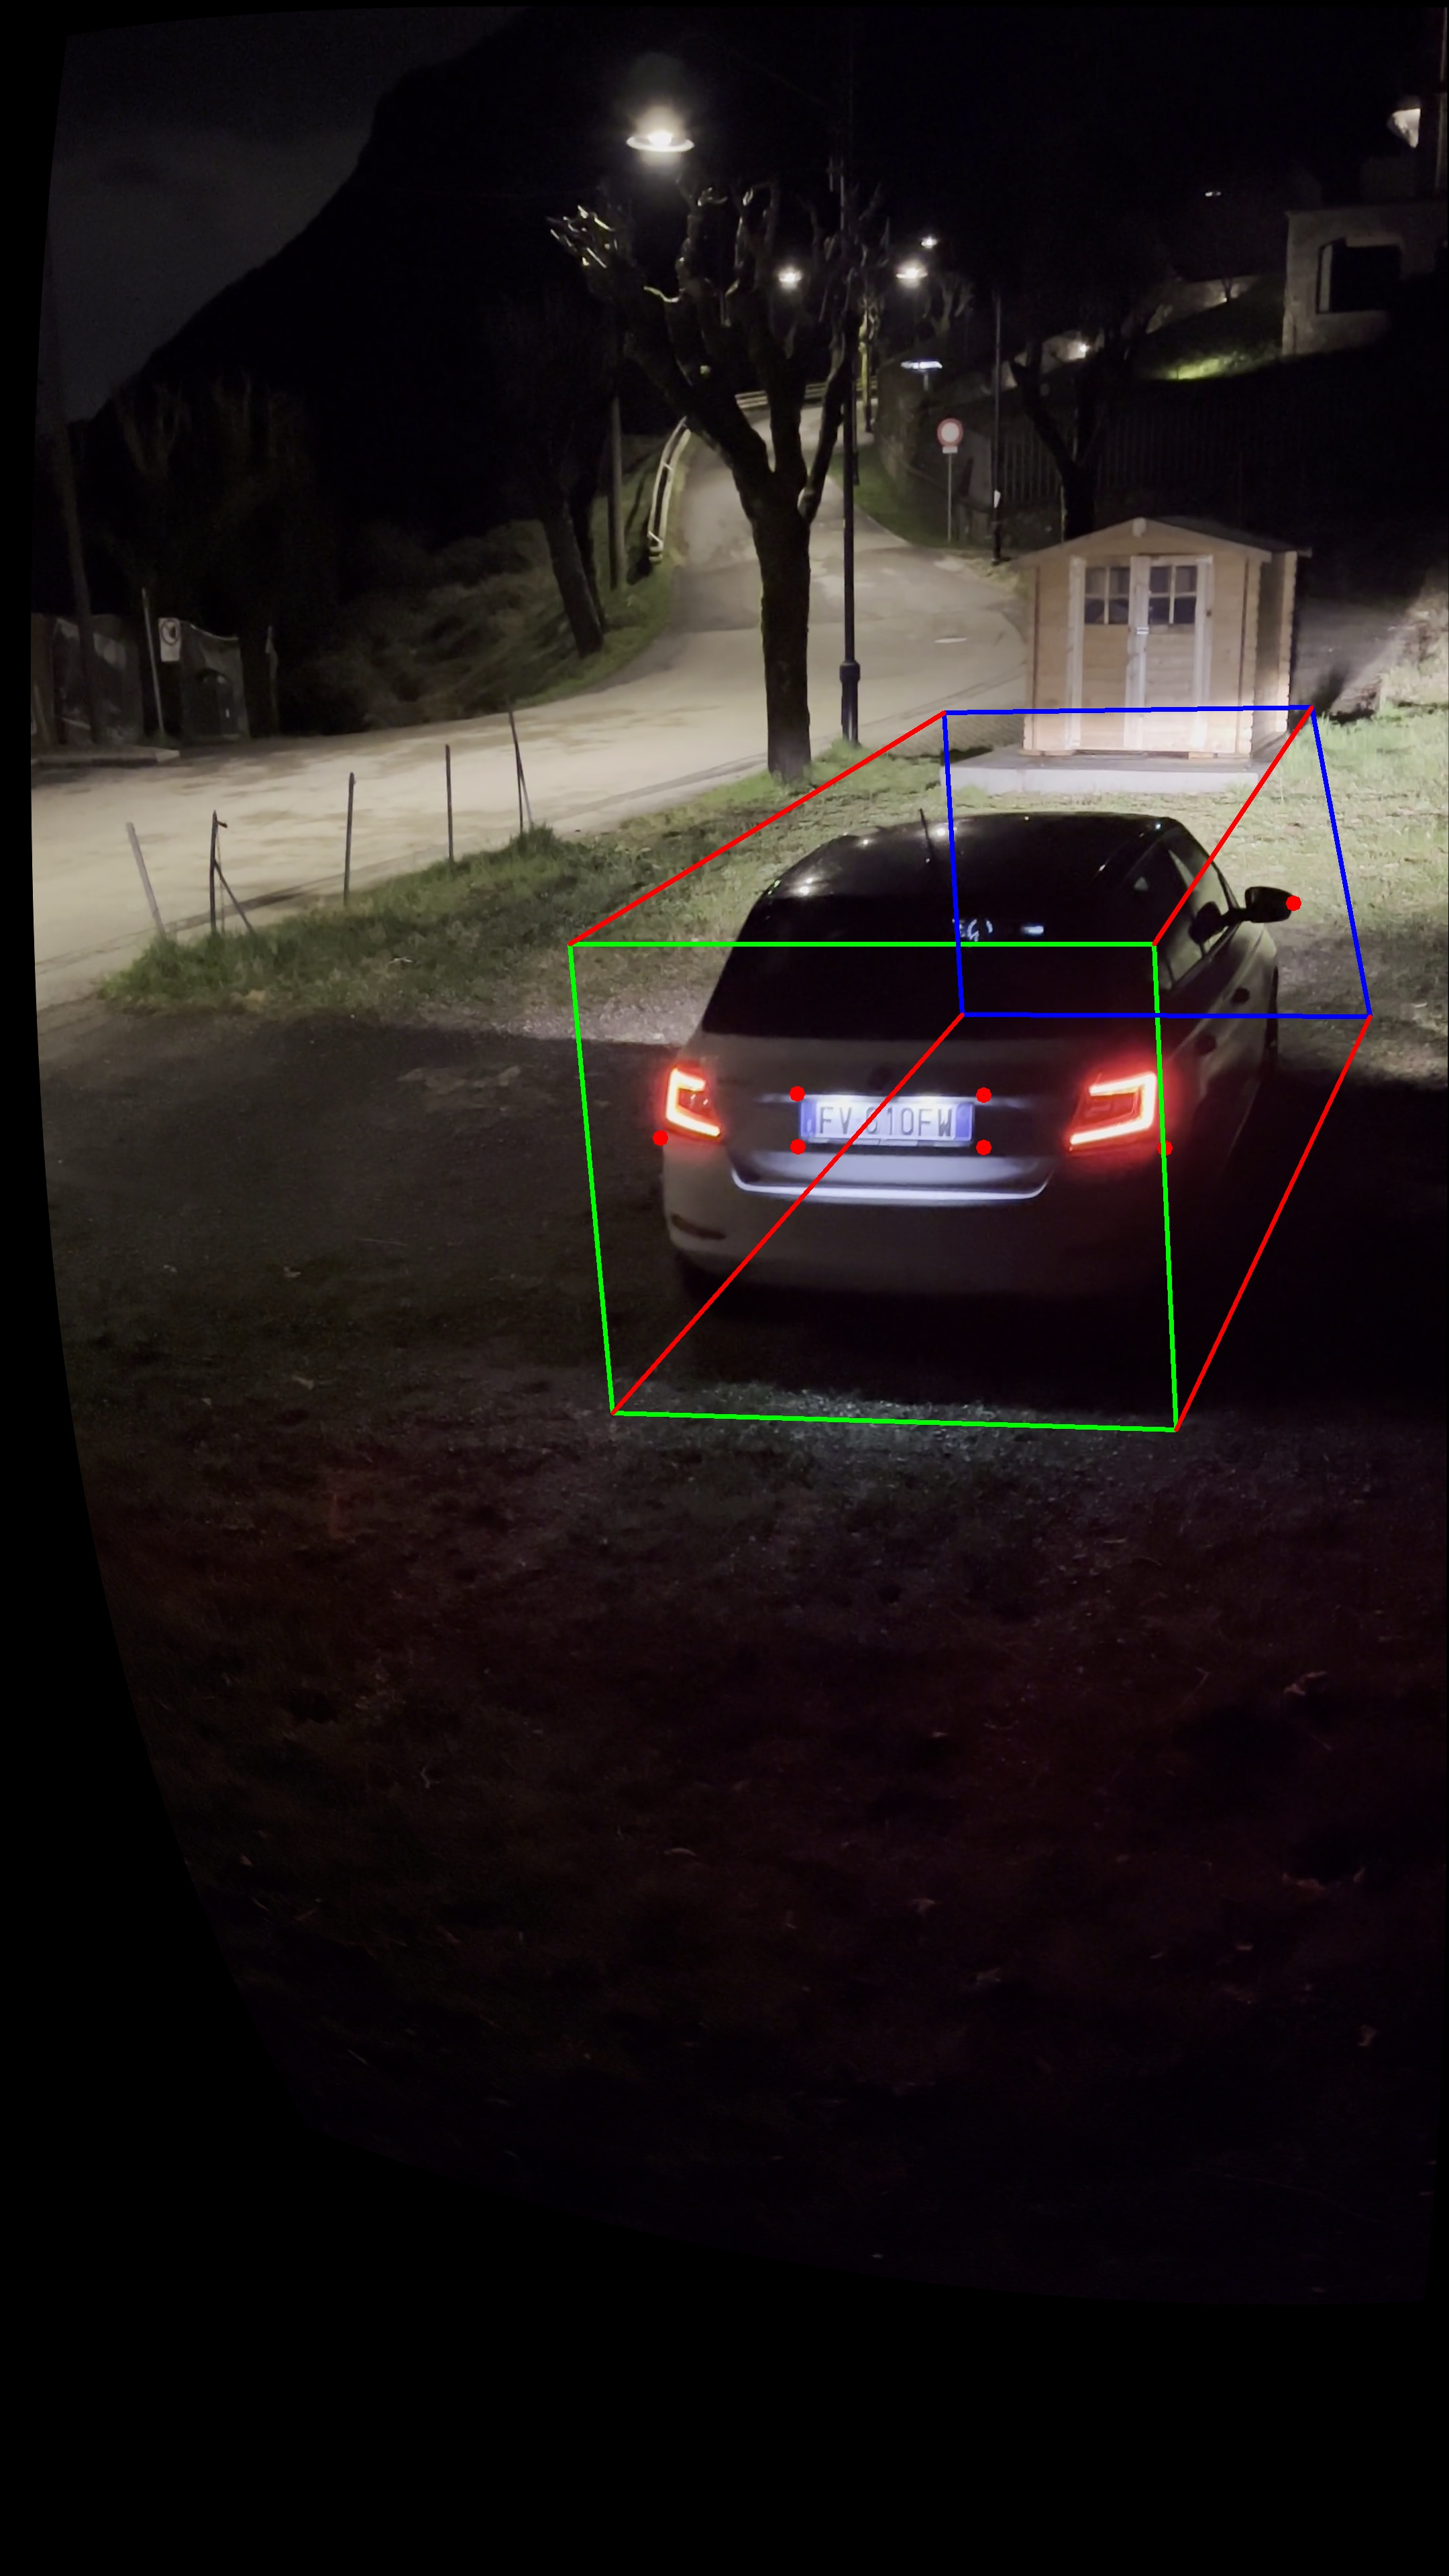
\includegraphics[width=0.20\textwidth]{Images/Conclusions/method4/4_frame8.jpg} &
        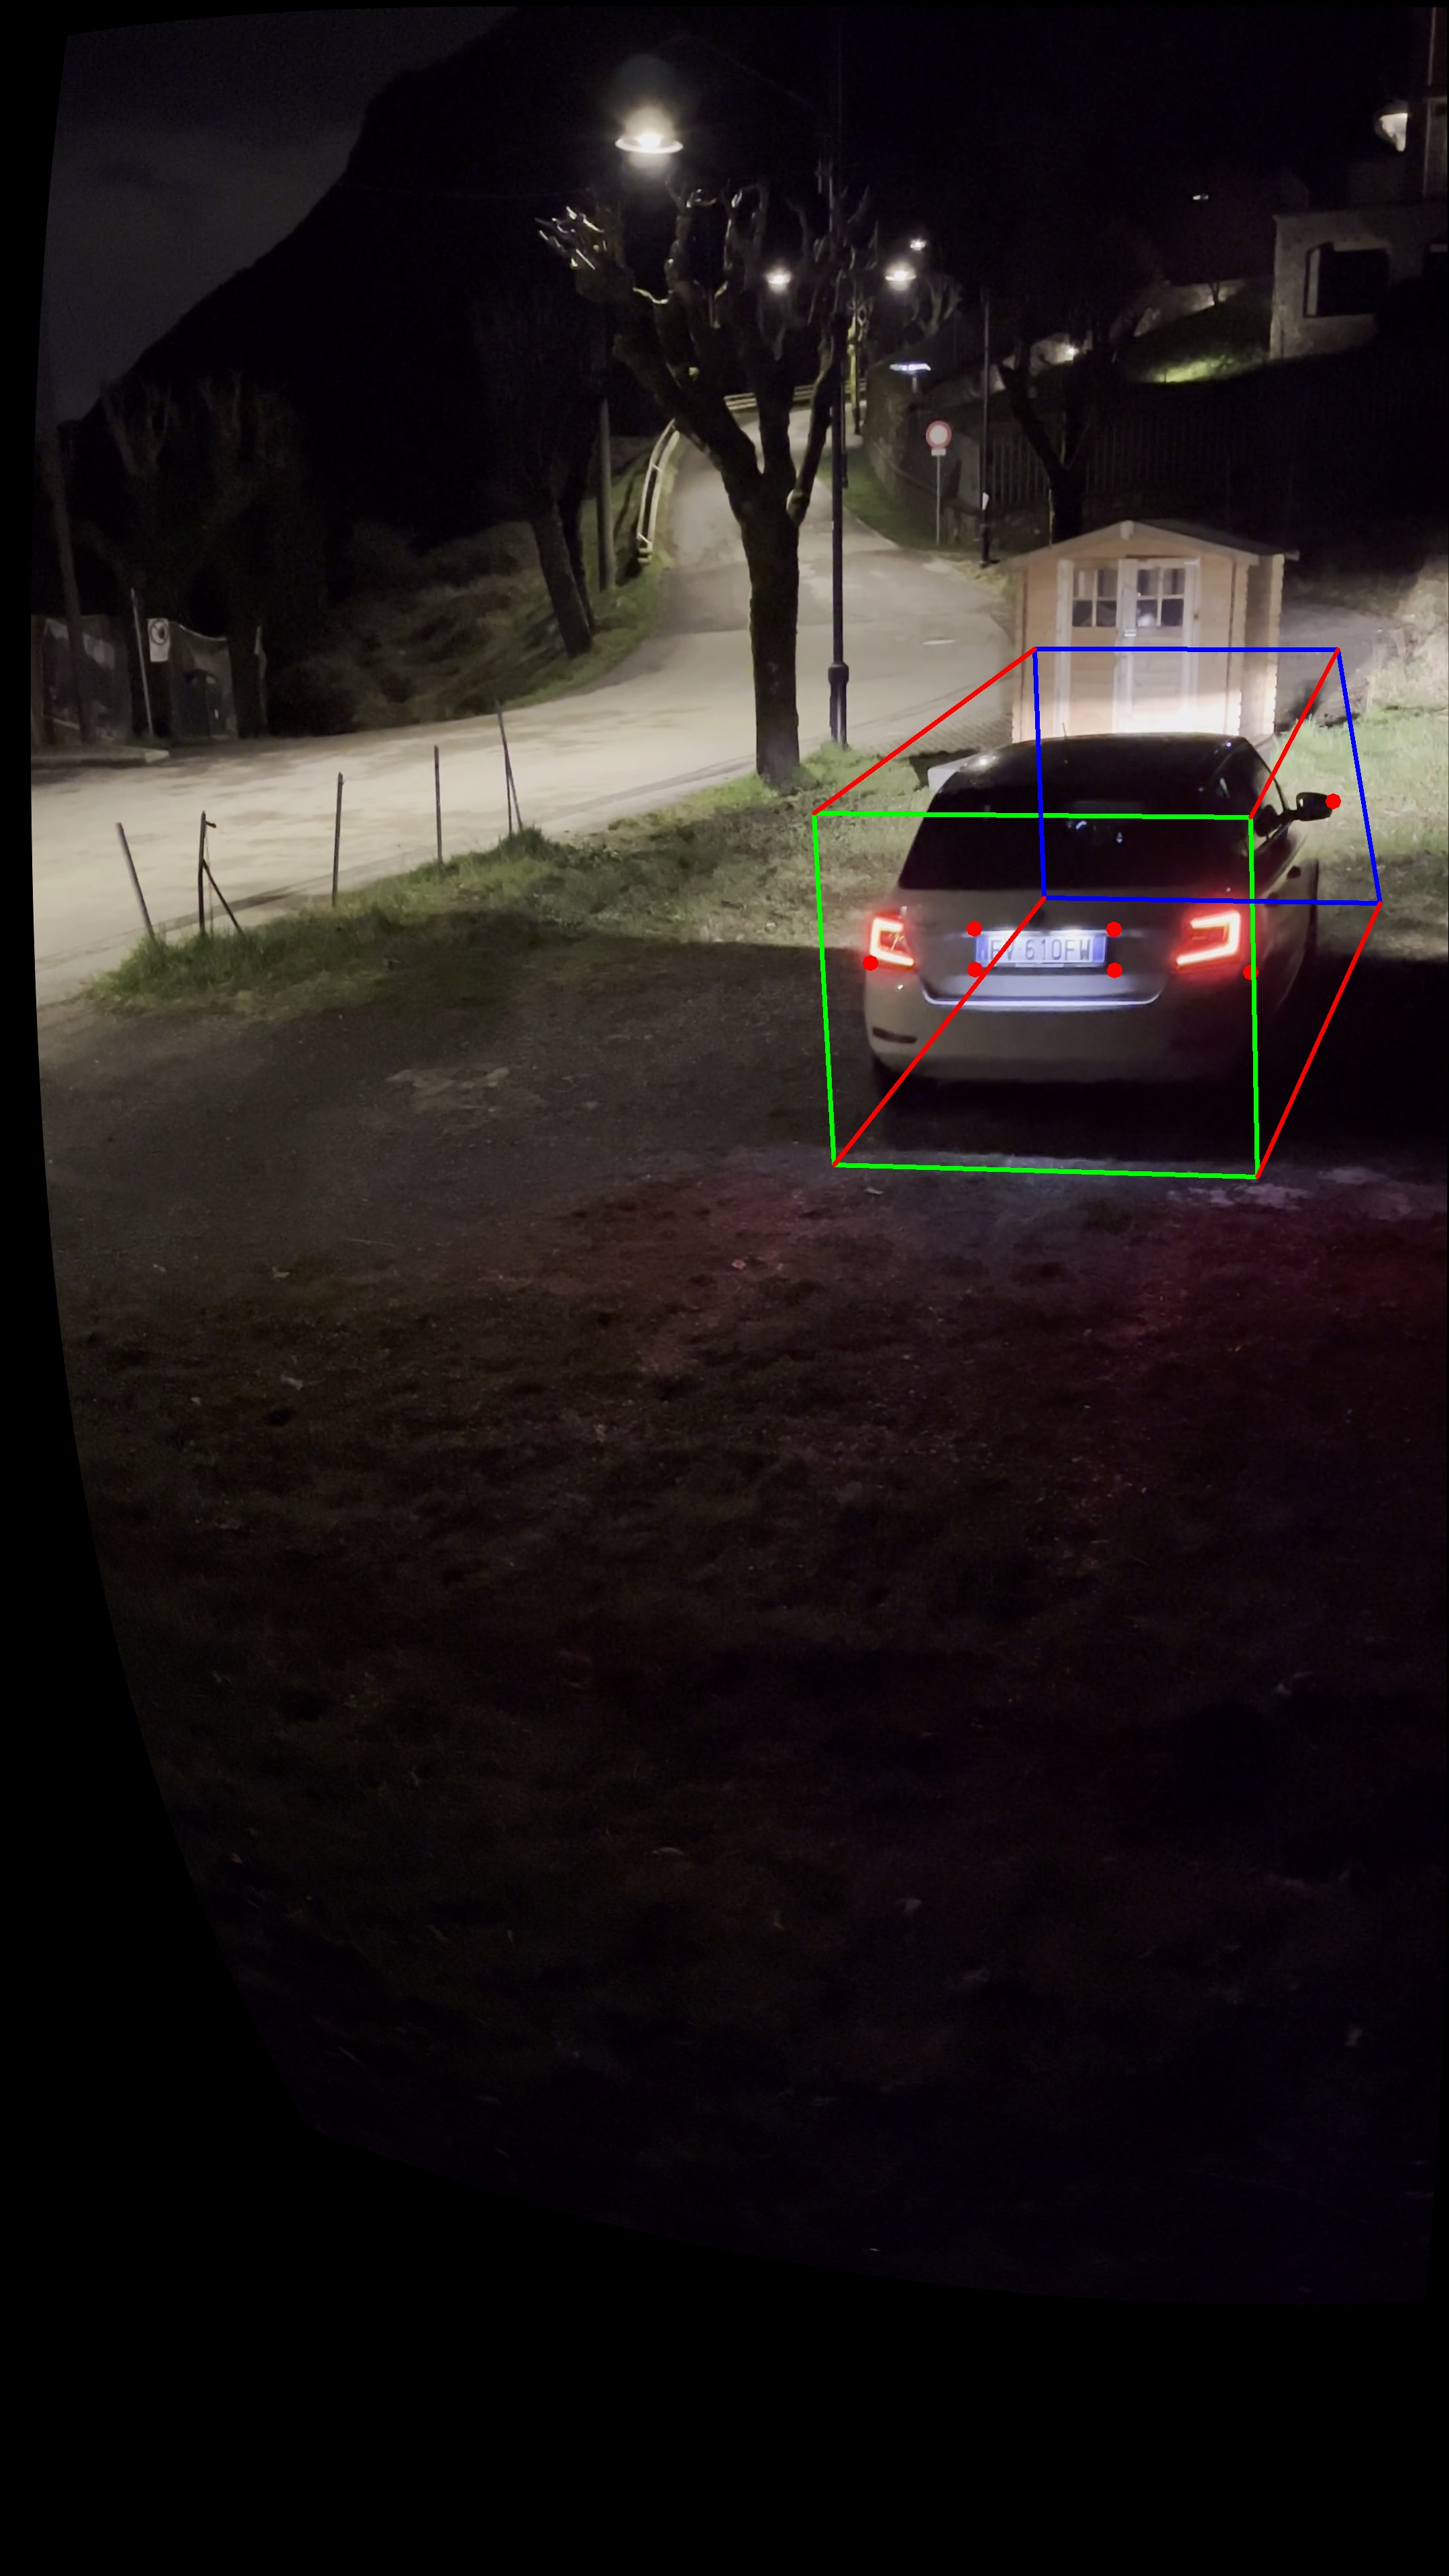
\includegraphics[width=0.20\textwidth]{Images/Conclusions/method4/4_frame12.jpg} &
        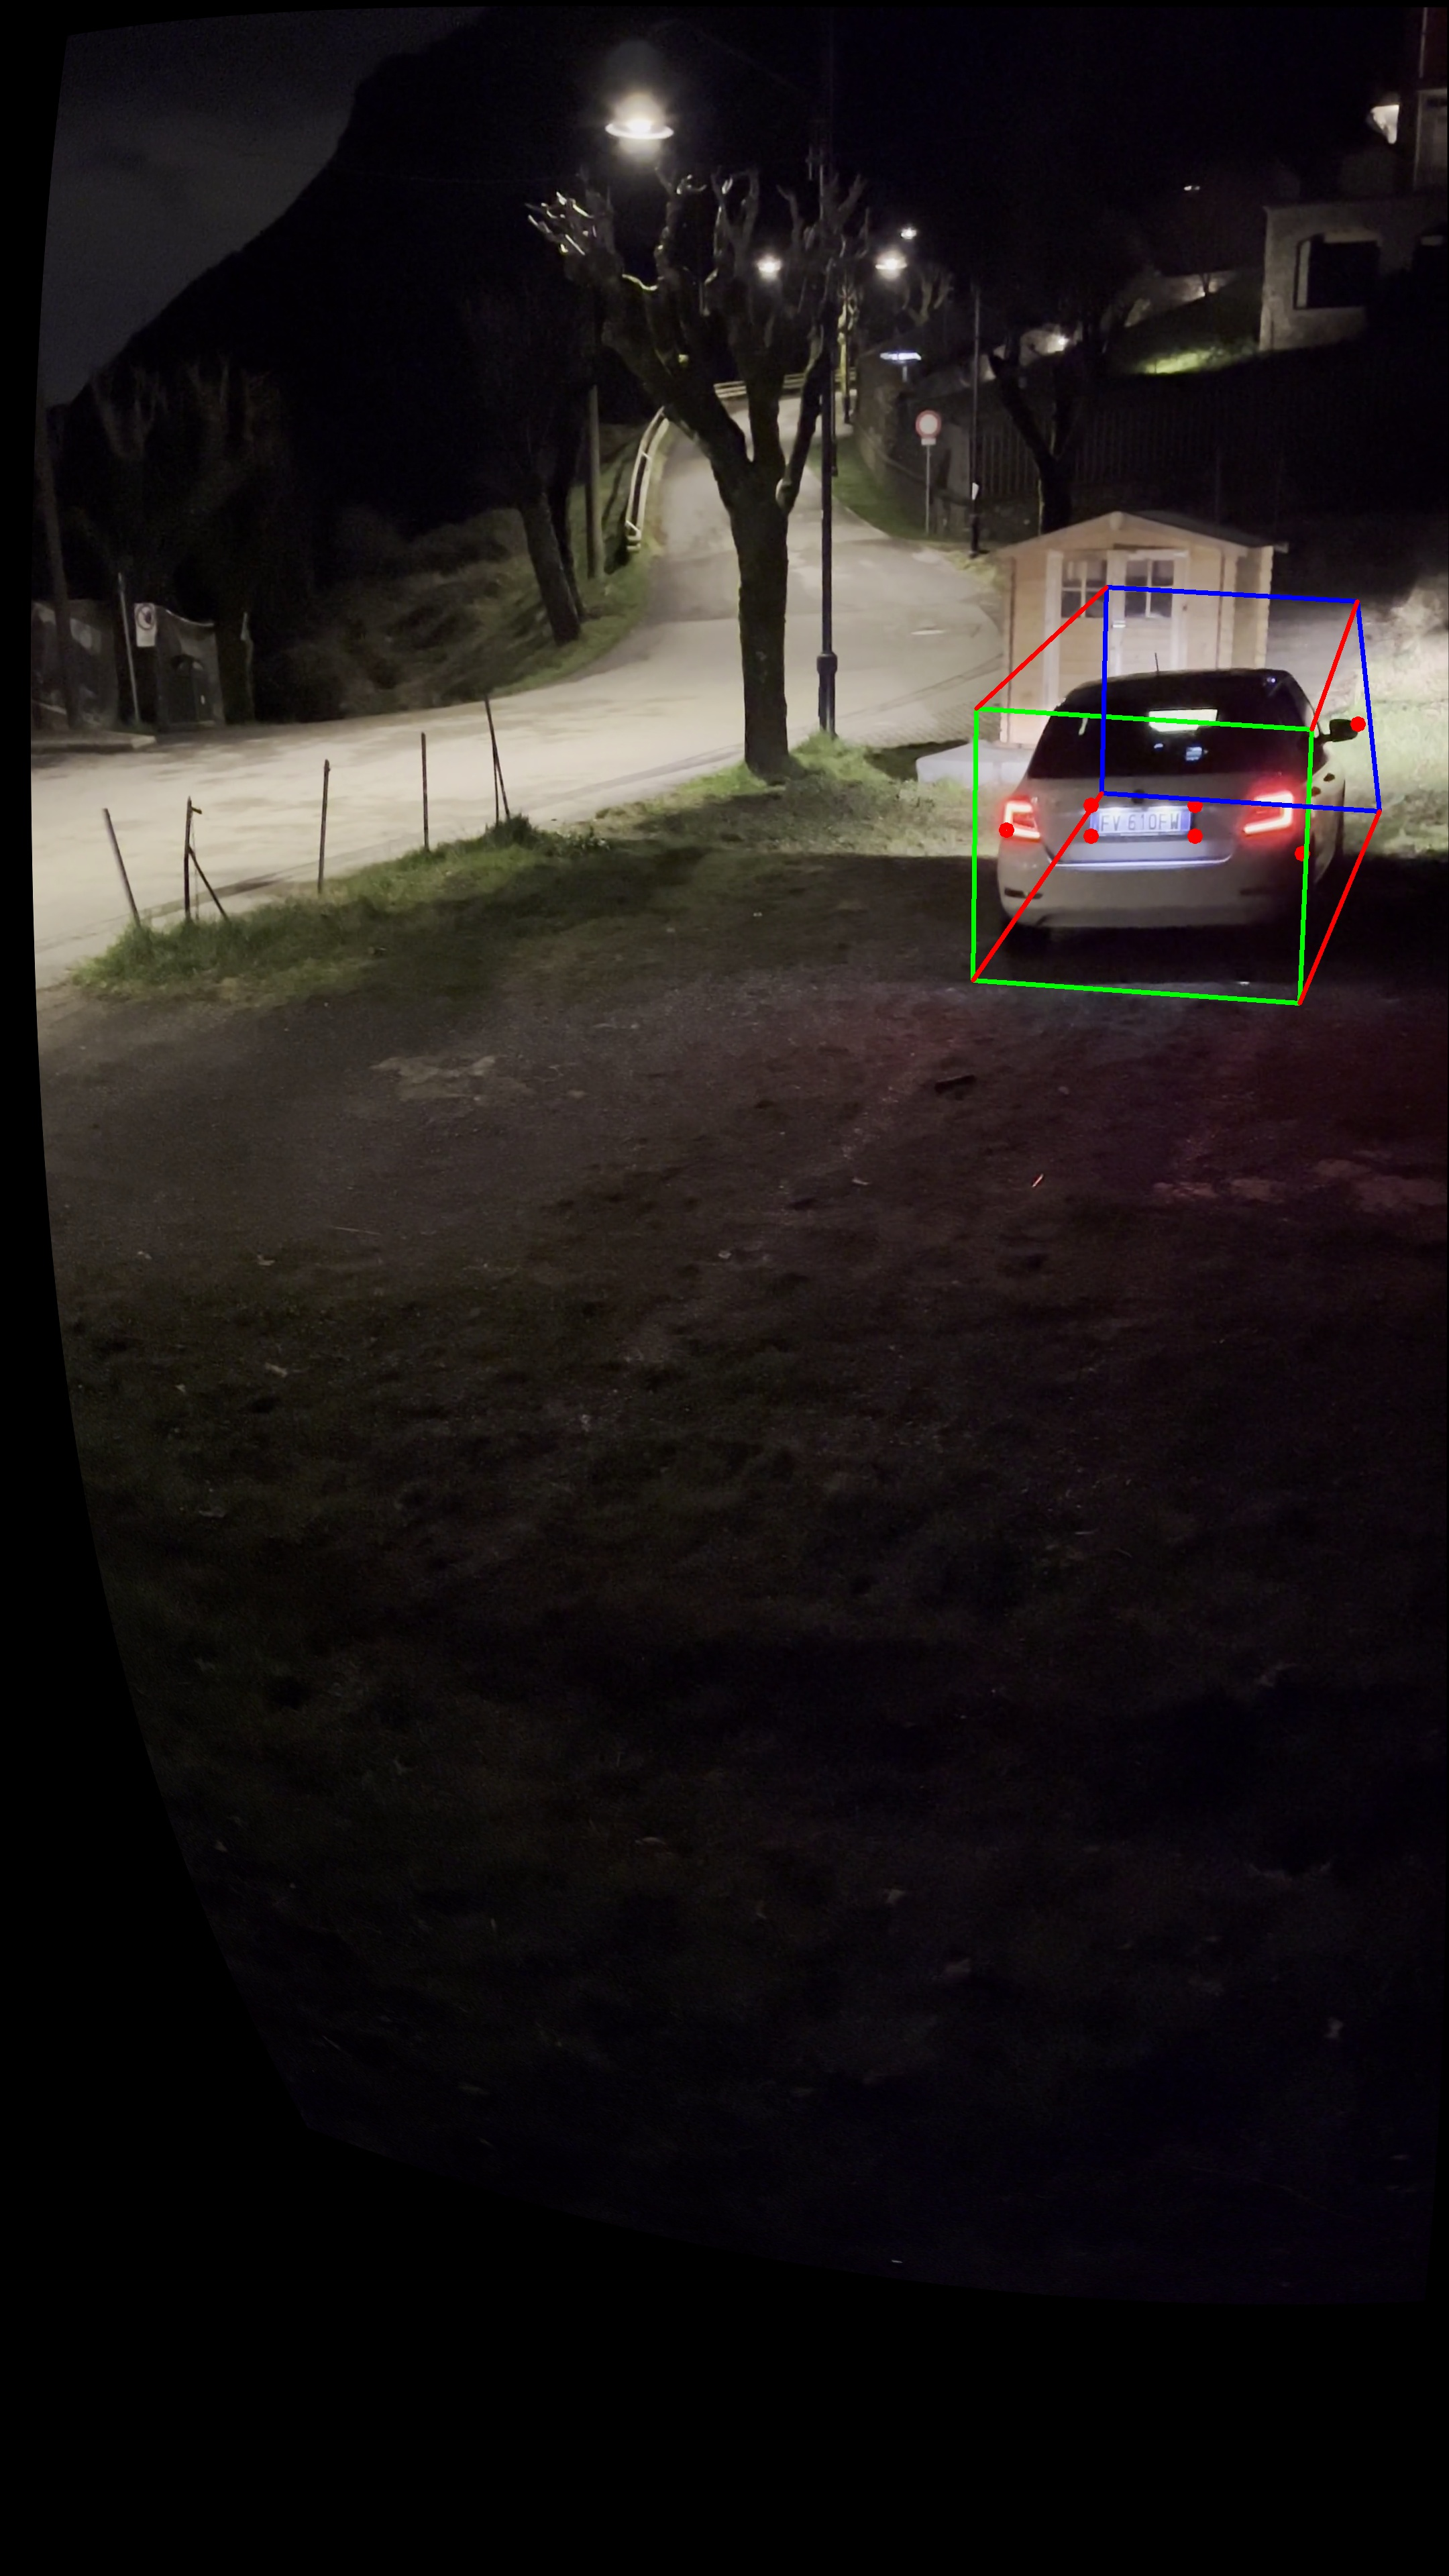
\includegraphics[width=0.20\textwidth]{Images/Conclusions/method4/4_frame16.jpg} \\
    \end{tabular}
    \caption{Comparison of results from different methods across four selected frames}
    \label{fig:grid_images}
\end{figure}


\section{Future Work}

Future work will aim to automate the retrieval of vehicle data by implementing a neural network to recognize license plate characters. The recognized plate will be used to query public databases to obtain the car's make and model. This information will then allow access to 3D CAD model repositories, providing accurate geometrical data without manual input. Additionally, improvements will be made to the robustness of license plate and light detection, using more advanced object detection algorithms to handle challenging conditions such as occlusion or low visibility.

